\documentclass[a4paper,twoside]{article}

\usepackage{epsfig}
\usepackage{subfigure}
\usepackage{calc}
\usepackage{amssymb}
\usepackage{amstext}
\usepackage{amsmath}
\usepackage{amsthm}
\usepackage{multicol}
\usepackage{pslatex}

\usepackage{apalike}

\usepackage{lipsum}  

\usepackage{balance}
\usepackage{graphicx}
\usepackage{caption}
%\usepackage{subcaption}
\usepackage{hyperref}
\usepackage[T1]{fontenc}
\usepackage[table,xcdraw]{xcolor}


\usepackage{SCITEPRESS}     % Please add other packages that you may need BEFORE the SCITEPRESS.sty package.

\subfigtopskip=0pt
\subfigcapskip=0pt
\subfigbottomskip=0pt


\newif\ifreview
%\reviewtrue
\reviewfalse

\begin{document}

\title{Modeling Semantics for Building Deconstruction}

\ifreview

\author{\authorname{ 
X.~Xxxxxx\sup{2}, 
X.~Xxxxx\sup{2},  
X.~Xxxxxxxx\sup{1},
X.~Xxxxxxx\sup{1}, 
X.~Xxxxxx\sup{1}, 
X.~Xxxxxxx\sup{3},
X.~Xxxxxxxxx\sup{3}
}
\affiliation{\sup{1}Department of Mathematics and Physics, Xxxx Xxx University, Xxxx, Xxxxx}
\affiliation{\sup{2}Department of Engineering, Xxxx Xxx University, Xxxx, Xxxxx}
\affiliation{\sup{3}XXXXXX X.x.X., Xxxx, Xxxxx}
\email{\{xxxxxx, xxxxxxxx, xxxxxx, xxxxx, xxxxxx\}@xxx.xxxxxxxx.xx, \{xxxxxxxx, xxxxxxxxxx\}@xxxxxx.xx}
}

\newcommand{\acks}{Partially supported by grant from XXXXXX X.x.X., a web service company owned by Xxxxx X.x.X. and XXXxXX ---  the ICT company of the Xxxxxx Xxxxxxx of Xxxxxxx and Xxxxxxx and the  Xxxxxxx Xxxxxxxx Xxxxx of Xxxxxxxx Xxxxxxxxx, respectively.}

\else

\author{\authorname{
E.~Marino\sup{2},
F.~Spini\sup{2},
D.~Salvati\sup{1},
C.~Vadal\`a\sup{1},
M.~Vicentino\sup{3},
A.~Paoluzzi\sup{1},
A.~Bottaro\sup{3}
}
\affiliation{\sup{1}Department of Mathematics and Physics, Roma Tre University, Rome, Italy}
\affiliation{\sup{2}Department of Engineering, Roma Tre University, Rome, Italy}
\affiliation{\sup{3}GEOWEB S.p.A., Rome, Italy}
\email{\{marino, spini, salvati, vadala, paoluzzi\}@ing.uniroma3.it, \{mvicentino, abottaro\}@geoweb.it}
}

\newcommand{\acks}{Partially supported by grant from GEOWEB S.p.A., a web service company owned by Sogei S.p.A. and CNGeGL ---  the ICT company of the Italian Ministry of Economy and Finance and the Italian National Board of Quantity Surveyors, respectively.}

\fi

\keywords{Building modeling, BIM, Deconstruction Semantics}

\abstract{
In this paper we discuss the motivation, the technology, the design and the use-model of a novel web service for quantity surveyors, aiming to exploit virtual and augmented reality methods to implement a ``zero waste'' model, i.e. a new design paradigm where the waste materials from demolition become resources for reconstruction. The goal of this project is to provide virtual/augmented reality tools through quick modeling of buildings and their fast augmentation with semantic content.
}

\onecolumn \maketitle \normalsize \vfill


%\section{\uppercase{Introduction}}
\label{sec:introduction}


A tendency to move away from the humanization of territories and to reuse already  built accommodation or accommodation which has fallen into disuse has become a pressing need in advanced societies. We have to integrate the ``zero energy'' model (each building has to produce the same amount of energy that it consumes) with the ``zero waste'' model , i.e. a new design paradigm where the waste materials from demolition become resources for reconstruction~\cite{altamura:12}. Building processes and designs have to be renewed to take account of environmental concerns. 

To reduce the impact of construction projects on the environment, the design needs to take the issue of building materials into consideration. Public administrations need suitable tools for the calculation and the control of reused or disposed materials. The new tools should handle the digital processing of materials throughout the project, supporting new project requirements such as: Design for Deconstruction, Design for Recycling and Design for Waste. In particular, a building life cycle, underpinned by a construction process which envisages cycles aligned to natural phenomena is the focus of this paper. 

In this work\footnote{\acks} we propose solutions that serve to close the circle of the building life-cycle, moving away from a traditional linear response with excessively high consumption energy rates (cradle to grave) and towards the reuse of materials in deconstruction/reconstruction (cradle to cradle), supported by computer aided selective demolition process.

All restructuring cycles should envisage de-construction and re-construction steps targeted towards the replacement of materials in order to achieve greater efficiency. The handling of these materials would require appropriate encoding both for the disposal (ECW - European Coding of Waste) and for the planning and design of new buildings (BIM --- Building Information Modeling). For this reason we need geo-referenced scenes of augmented reality based on fast, easily navigable and measurable 3D models. 

We already have excellent knowledge about construction costs (from scratch) but little is known about replacement rates (complete selective demolition). A modern selective demolition process requires human intervention, with high insurance costs due to the danger involved for those working in these activities. This latter point demands an alternative to human effort in these process. We suggest that automated robots could replace human effort; these drones could operate in a semantically familiar context and give real-time updates as the reality contextually changes. 

We believe, therefore, that there is a big need for modern and easy-to-use modeling frameworks for building deconstruction in the AEC industry, to enable an augmented reality through semantic recognition by computer vision and by photogrammetric precision up to centimetric definition. Such virtual/augmented reality tools require both fast 3D building modeling and augmentation with semantic content, in order to be controlled in almost real time: this real challenge is also required by the future development of IoT. 	  
 
In this section we have discussed the motivation of the project described in this paper. The remaining sections are organized as follows.
Section~\ref{sec:deconstruction} introduces a more technical viewpoint about the state of deconstruction topics in Europe and in Italy.
Section~\ref{sec:application} describes the client application and the proposed workflow for quantity surveyors.
Section~\ref{sec:architecture} illustrates the framework architecture. 
Section~\ref{sec:modeling} shortly recalls the methodology, programming style and environment of our geometric computing approach to solid modeling.
In the conclusion section we outline the work to be done and provide our forecast about possible developments.

\section{\uppercase{Introduction}}
\label{sec:introduction}

\noindent
A tendency to minimize the humanization of new territories and to push for reusing already  built accommodation or accommodation which has fallen into disuse has become a pressing need in advanced societies. We have to integrate the ``zero energy'' model (each building has to produce the same amount of energy that it consumes) with the ``zero waste'' model, i.e. a new design paradigm where the waste materials from demolition become resources for reconstruction~\cite{altamura:12}. Building, contract, and design processes need to be renewed to take account of environmental concerns. 

To reduce the impact of construction projects on the environment, the design needs to take the issue of building materials into consideration. Public administrations need suitable tools for the calculation and the control of reused or disposed materials. The new tools should handle the digital processing of materials throughout the project life cycle, supporting new project requirements such as: Design for Deconstruction, Design for Recycling and Design for Waste. 

In particular, a building life cycle, underpinned by a construction process which envisages cycles aligned to natural phenomena is the focus of this paper. 

In this work\footnote{\acks} we propose solutions that serve to close the circle of the building life-cycle, moving away from a traditional linear response with excessively high consumption energy rates (cradle to grave) and towards the reuse of materials in deconstruction/reconstruction (cradle to cradle), supported by computer aided selective demolition process.

All restructuring cycles of buildings should envisage de-construction and re-construction steps, targeted towards the replacement of materials in order to achieve greater efficiency. The handling of these materials requires appropriate encoding both for the disposal, according to EWC (European Waste Catalogue) codes, and for the planning and design of new buildings, following BIM (Building Information Modeling) methodology. For this purpose we need geo-referenced scenes of augmented reality based on fast, easily navigable and measurable 3D models. 

We already have excellent knowledge about construction costs (from scratch) but little is known about replacement rates (complete selective demolition). A modern selective demolition process requires human intervention, with high insurance costs due to the danger involved for those working in these activities. This latter point demands an alternative to human effort in these process. We suggest that automated robots could replace human effort; drones could operate in a semantically familiar context and give real-time updates as the reality contextually changes. 

We believe, therefore, that there is a big need for modern and easy-to-use modeling frameworks for building deconstruction in the AEC (Architecture, Engineering and Construction) industry, to enable an augmented reality through semantic recognition by computer vision and by photogrammetric precision up to centimetric definition. Such virtual/augmented reality tools require both fast 3D building modeling and augmentation with semantic content, in order to be controlled in almost real time: this real challenge is also required by the future development of the Internet of Things. 	  
 
In this section we have discussed the motivation of the project described in this paper. The remaining sections are organized as follows.
Section~\ref{sec:deconstruction} introduces a more technical viewpoint about the state of deconstruction topics in Europe and in Italy.
Section~\ref{sec:application} describes the client application and the proposed workflow for quantity surveyors.
Section~\ref{sec:architecture} illustrates the framework architecture. 
Section~\ref{sec:modeling} shortly recalls the methodology, programming style and computational environment of our geometric programming approach to solid modeling.
In the conclusion section we outline the work to be done and provide our forecast about possible developments.


%\section{\uppercase{BIM and Design for Deconstruction}}
\label{sec:deconstruction}


\subsection{Regulatory framework}

Waste management is an issue that in recent decades has become increasingly more important, considering its economic, environmental and energy  impact.
The European Community has defined standards (EU 98/2008, 1357/2014) and goals (qualitative and quantitative) that Member States must comply with through the enactment of national regulations and the definition of economic instruments.

Waste disposal, with direct and indirect costs involved, is enforced by Construction and Demolition activities. In European Waste Code/Classification (CER) [955/2014 EU] waste from the demolition of buildings are identified as class 17 -- Construction And Demolition Wastes (including Excavated Soil From Contaminated Sites). 
This classification allows a correct identification of both the waste generated from adoptable demolition modes, and the waste produced by actions of re-use, recycling or landfilling.
 
The regulatory framework for waste management is far from clear, in particular in the national context. Despite the cost of the "landfill", this is often preferred rather than risking administrative or criminal penalties for failure to comply with unclear rules.  


\subsection{Proposed approach}




E` all’interno di questo quadro normativo che rischia di essere farraginoso che riteniamo utile promuovere l’utilizzo di strumenti (di supporto) che, grazie una modellazione 3D dell’edificio capace di integrare anche una descrizione semantica delle parti che lo compongono e delle loro relazioni, possano favorire il superamento delle difficoltà amministrative come pure l’efficacia nella corretta identificazione dei rifiuti prodotti, e quindi delle opportune scelte fra le possibili azioni virtuose, ovvero quelle di recupero e di riuso.

A cui si aggiunge, in contesto di modellazione, la possibilità di identificare in modo puntuale i costi, così come i possibili ricavi derivanti dal percorso alternativo di riciclo/riuso rispetto allo smaltimento, oltre che la composizione e integrazione di informazioni utili alla pianificazione delle attività di cantiere.
 
Inoltre, in un ambiente di modellazione e calcolo, si rende possibile sia la verifica del raggiungimento delle soglie di riuso/recupero previste dalle normative (una sorta di validazione dell’intervento sul cantiere) che anche la possibilità di confrontare fra loro diverse opzioni  





*** Spunti da sviluppare (?)

Uno strumento di editing ---veloce--- rende percorribile la strada di adempiere agli obblighi di legge

Dall’abstract di questo articolo Building Information Modeling (BIM) for existing buildings — Literature review and future needs (\url{www.sciencedirect.
com/science/article/pii/S092658051300191X }) 

mi sembra interessante la seguente lista di cose 

Results show scarce BIM implementation in existing buildings yet, due to challenges of 

(1) high modeling/conversion effort from captured building data into semantic BIM objects, 

(2) updating of information in BIM and 

(3) handling of uncertain data, objects and relations in BIM occurring in existing buildings.


dati circa lo elevato costo sociale, ambientale e economico delle materie prime utilizzate in edilizia .

il 10-15\% consumi energetici del settore C\&D si deve alla estrazione delle materie prime (Rapporto United Nations Environment Programme: Buildings and Climate Change 2002)

il 25\% dei rifiuti prodotti (in Italia) deriva dal settore C\&D

 
\section{\uppercase{Design to Deconstruct}}
\label{sec:deconstruction}

\noindent 
Waste management is an issue that in recent decades has become increasingly important, considering its economic, environmental and energy  impact.

\subsection{Regulatory framework}
\label{sec:CER}

\noindent
The European Community has defined standards [EU 98/2008, 1357/2014] and goals (qualitative and quantitative) that Member States must comply with through the enactment of national regulations and the definition of economic instruments.

Waste disposal, with direct and indirect costs involved, is enforced by Construction and Demolition activities. In EWC, waste from the demolition of buildings [955/2014 EU] are identified as class 17 -- Construction And Demolition Wastes.
This classification allows a correct identification of both the waste generated from adoptable demolition modes, and the waste produced by actions of re-use, recycling or landfilling.
 
The regulatory framework for waste management is far from clear, in particular in the Italian national context. Despite its direct and indirect costs, the landfill is often preferred rather than risking administrative or criminal penalties for failure to comply with unclear rules.

\subsection{Proposed approach}

\noindent
Given this cumbersome regulatory framework, our project is promoting the use of simplified IT tools to support the deconstruction. In particular, a quick simplified geometric modeling of the building allows for integration of a semantic description of component parts and their materials. Virtual/Augmented Reality  strongly helps overcome the administrative difficulties, provided the correct identification of the waste produced.
This approach will increase the adoption of virtuous actions, namely the recovery and reuse.

In particular, a  geometric modeling of the building allows to identify:
(a) cost / income resulting from alternatives of recycling / re-using instead of disposal;
(b) the composition and integration of information useful to the planning of construction activities;
(c) achievement of the thresholds of reuse / recovery required by the regulations;
(d) ability to economically compare different options.

We started by considering the SMARTWaste system~\cite{smartWaste}. Their approach allows to derive estimates of the quantities of materials by providing a description of the type of building and the area where it was built. With this information, the forms that provide an aggregated representation of the data of interest are automatically filled.

Our approach to deconstruction conversely provides both a geometric modeling of building subsystems and components and a semantic annotation with construction materials, like a sort of \emph{simplified} BIM. As a matter of fact, our national construction industry is strongly heterogeneous, so that  we need a pretty detailed modeling to obtain enough accurate information.
One vantage point of this approach is an incremental iterative character, where each modeling stage may be followed by validation of partial costs.

A complete report about using BIM as a building deconstruction approach is provided by~\cite{galic2014bim}. A study on the usage of BIM as a support for Design for Deconstruction is carried on by~\cite{akinade2015waste}. In this setup, on the contrary to what holds for us, deconstruction has to be a major concern starting from the beginning of the building design.

A large corpus of specialized literature exists about BIM for existing buildings. A very interesting review paper, discussing hundreds of references is~\cite{Volk2014109}. Its abstract states that:  ``While BIM processes are established for new buildings, the majority of existing buildings is not maintained, refurbished or deconstructed with BIM yet. Promising benefits of efficient resource management motivate research to overcome uncertainties of building condition and deficient documentation prevalent in existing buildings.'' 

The \emph{Metior} (from Latin: to  \emph{measure} or  \emph{estimate}) project, introduced in this paper, is exactly aiming to overcome such difficulties, via (a)~the design and implementation of a \emph{web service} providing a strongly simplified user-interface, designed for quantity surveyors; (b)~storing a growing database of template plugins for more geometrically complex building parts; (c)~using an extensible geometry engine and server based on decades of research; (d)~offering flexible semantic additions via specialization of IFC (Industry Foundation Classes~\cite{ifc}) classes associated to building subsystems and parts.

Metior specifically targets quantity surveyors. In fact, although large sites to be deconstructed are operated by main contractors, where skills and specific tools might be widely available and already used, most of deconstruction activities, and hence the largest amount of waste material produced, are managed by quantity surveyors from small or medium companies --- or even by single professionals. Such kind of firms may need to be supported with tools where the complexity, both bureaucratic and technical, have to be hidden although correctly managed.


%\vspace{-2mm}
\section{\uppercase{Deconstruction App}}
\label{sec:application}
\vspace{-2mm}

\noindent
A deconstruction oriented to the maximum reuse of materials must be supported by a \emph{workflow} that guides the user towards estimating the costs of the process. The aim is the determination of  \emph{building demolition costs}, depending also on transportation  and disposal of materials.

\vspace{-3mm}\subsection{Workflow}\vspace{-3mm}

\paragraph{Project definition} 

The first phase of the modeling process is a gross description of the building, in order to provide basic clues for a correct attribution of the semantic attributes.
In particular, we ask for: the apparent age, the style of construction, the historic use register, and the geolocation.
The estimated age and the style of construction are used to determine the needed data about the used materials; the record of use destinations allows you to to reconstruct the hazard notes of the items to be disposed of; geolocation finally allows to find out the recycling facilities closest to the site.

\vspace{-2mm}\paragraph{Building modeling} 
The user describes the construction using some predefined classes of elements, either instancing some  predefined parametric plugins or through wire-frame input of 2D layouts. 
First is defined the building skeleton (backbone), i.e.~the set of beams and columns or load-bearing walls, providing the structural grid.
On its horizontal sections, the user specifies the exterior and interior walls (vertical enclosure and partitions), on which the fixtures are positioned (horizontal communications).
Ceilings and floors (horizontal partitions) are instead automatically generated from the topology (1-boundary) of the 2-skeleton of the floors (subsets of 2-cells).
Finally, various elements such as stairs, elevators (vertical communications), foundations and roofs (horizontal enclosures) are placed, using ad-hoc templates interactively provided by Metior's plugin server, for appropriate sizing and part dimensioning.

\vspace{-2mm}\paragraph{Semantic annotations} 
At this stage the previously inserted elements are annotated semantically  by means of references to database of materials, including densities. The annotation may consists of one or more materials, including percentages.
For disposal control imposed by regulations, the user should assign one / more ECW codes and degrees of dangerousness (see Section~\ref{sec:CER}).
In this stage it is also assigned a pair of links that refer to the time schedule for disposal of  building components.

\begin{figure}[!h]
  \centering
  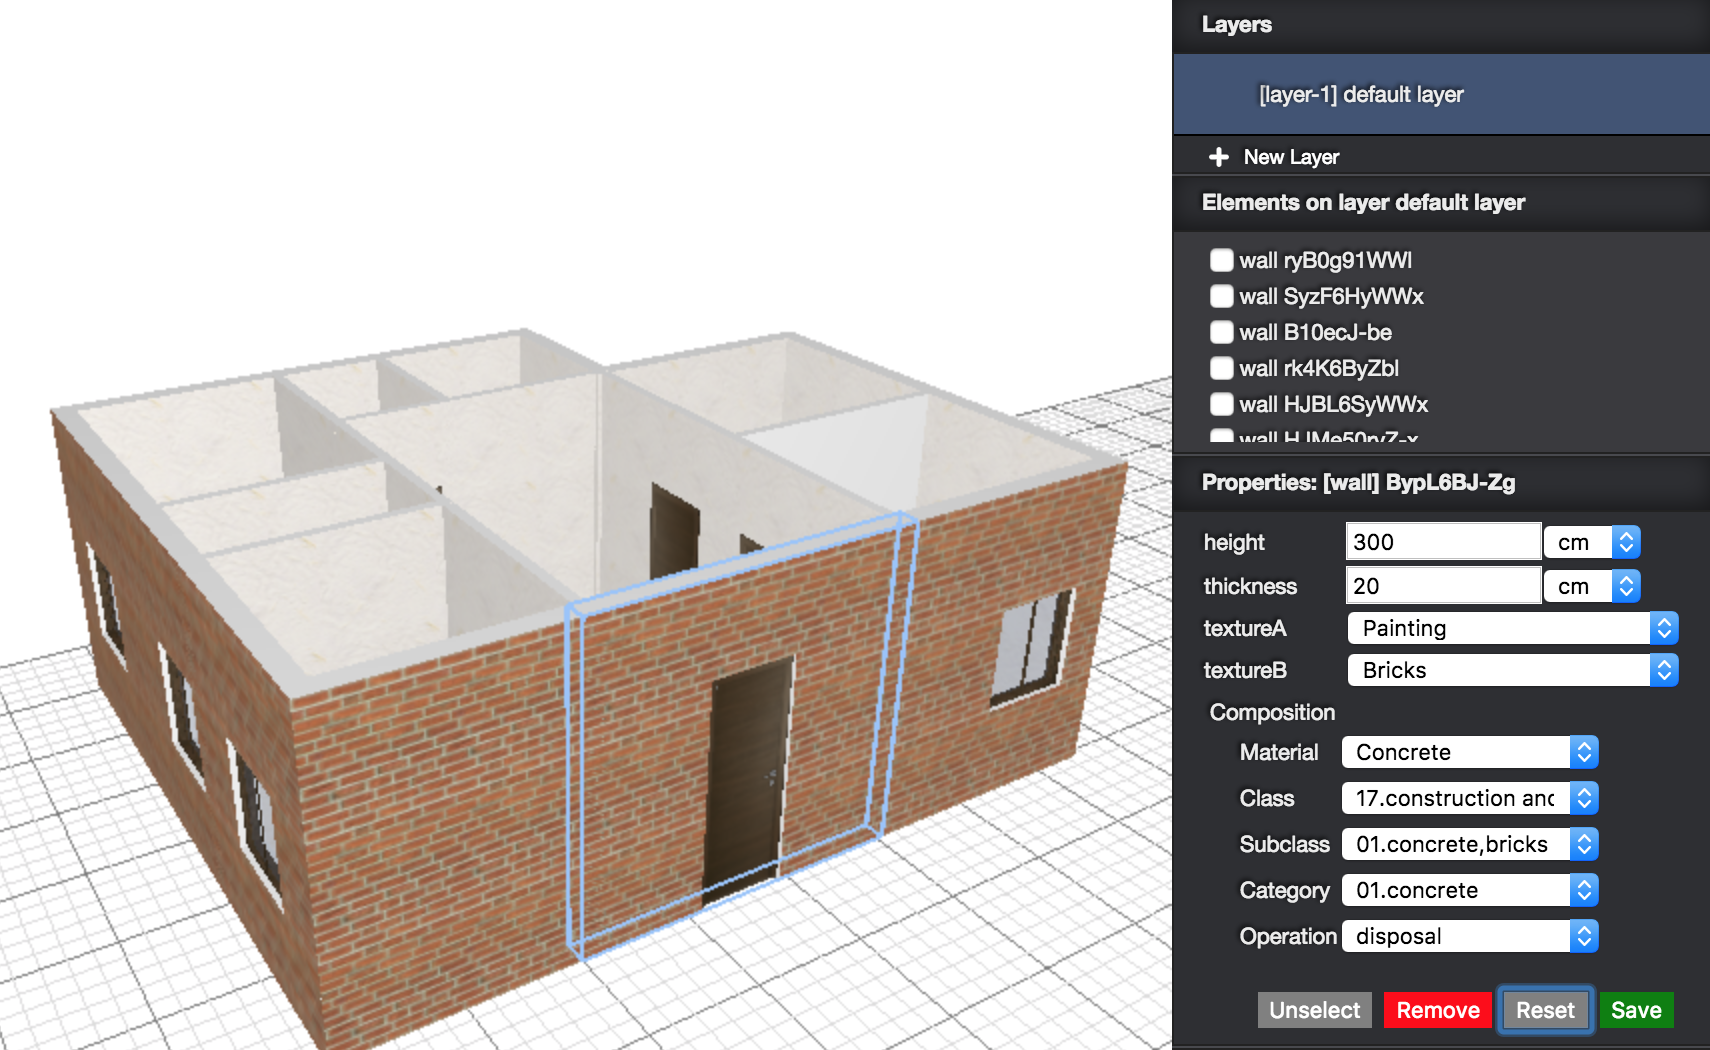
\includegraphics[width=1\linewidth]{images/3d-sel.png}
  \caption{Graphical interface for semantics annotation of a modeled object}
  \label{fig:semantics}
\end{figure}

\vspace{-2mm}\paragraph{Augmented reality visualization} 
After modeling and attribution of semantics to components, the quantity surveyer can validate the entire model by spatial merging into a 3D point cloud (see Figure~\ref{fig:augmented}) previously obtained by using flying drones for the exterior, or 3D laser scanners for the interior. In this way one can assess the adhesion of the modeled building structure to reality, possibly retracing to some previous step if the result is still not satisfactory.

\begin{figure}[htbp] %  figure placement: here, top, bottom, or page
   \centering
   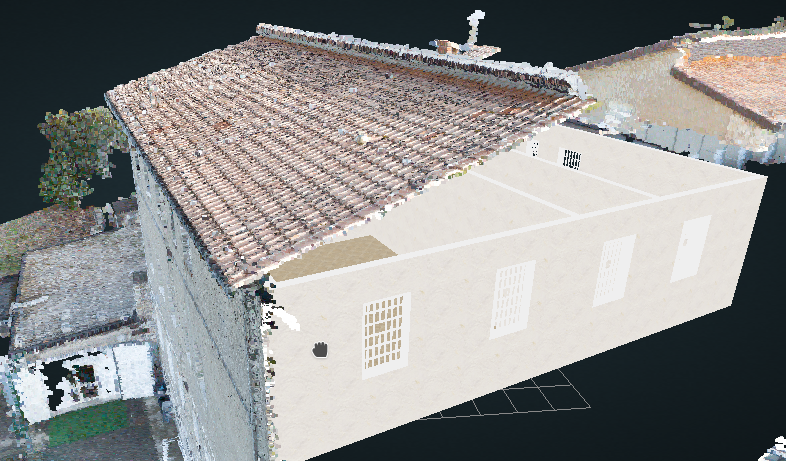
\includegraphics[width=1\linewidth]{images/augmented}
   \caption{A model inside a point cloud}
   \label{fig:augmented}
\end{figure}

\vspace{-3mm}\subsection{Process output}\vspace{-3mm}

\noindent 
Once the work is done and the model geometry is validated, the application provides a final report.
In particular, the final report will allows the quantity surveyer and/or the other professionals involved in the deconstruction design team, to determine whether the decision taken is convenient both economically and/or environmentally.

The final report consists of four documents.
(i)~\emph{An estimate of volumes and weights of materials}, computed by appropriate integration calculations, based on the geometry of components and annotations defined on them.
(ii)~\emph{An estimate of demolition costs}, including disposal and recovery.
Starting from volumes and densities of materials, and from ECW codes and hence the mode of disposal, it is estimated the cost of the contribution to landfills.
(iii)~\emph{The transportation costs} to move the materials to the closest landfills, taking into account the geographical position of the building, and by calculating the most convenient road routes.
(iv)~\emph{An estimate of the expected time} for the complete demolition of the building, located on a Gantt chart. A PERT program, automatically generated while annotating semantically the components of the building, is used for this purpose.

\noindent
\section{\uppercase{Deconstruction App}}
\label{sec:application}

\noindent
A deconstruction oriented to the maximum reuse of materials must be supported by a \emph{workflow} that guides the user towards estimating the costs of the process. The aim is the determination of  \emph{building demolition costs}, depending also on transportation  and disposal of materials.

\subsection{Workflow}

\paragraph{Project definition} 

\noindent
The first phase of the modeling process is a gross description of the building, in order to provide basic clues for a correct attribution of the semantic attributes.
In particular, we ask for: the apparent age, the style of construction, the historic use register, and the geolocation.
The estimated age and the style of construction are used to determine the needed data about the used materials; the record of use destinations allows to reconstruct the hazard notes of the items to be disposed of; geolocation finally allows to find out the recycling facilities closest to the site.

\paragraph{Building modeling} 

\noindent
The user describes the construction using some predefined classes of elements, either instantiating some  predefined parametric plugins or through wire-frame input of 2D layouts. 
First is defined the building skeleton (backbone), i.e.~the set of beams and columns or load-bearing walls, providing the structural grid.
On its horizontal sections, the user specifies the exterior and interior walls (vertical enclosure and partitions), on which the fixtures are positioned (horizontal communications).
Ceilings and floors (horizontal partitions) are instead automatically generated from the topology (1-boundary) of the 2-skeleton of the floors (subsets of 2-cells).
Finally, various elements such as stairs, elevators (vertical communications), foundations and roofs (horizontal enclosures) are placed, using ad-hoc templates interactively provided by Metior's plugin server, for appropriate sizing and part dimensioning.

\paragraph{Semantic annotations} 

\noindent
At this stage (see Figure~\ref{fig:semantics}) the previously inserted elements are annotated semantically  by means of references to database of materials, including densities. The annotation may consists of one or more materials, including percentages.
For disposal control imposed by regulations, the user should assign one / more EWC codes and degrees of dangerousness (see Section~\ref{sec:CER}).
In this stage it is also assigned a pair of links that refer to the time schedule for disposal of  building components.

\begin{figure}[!h]
  \centering
  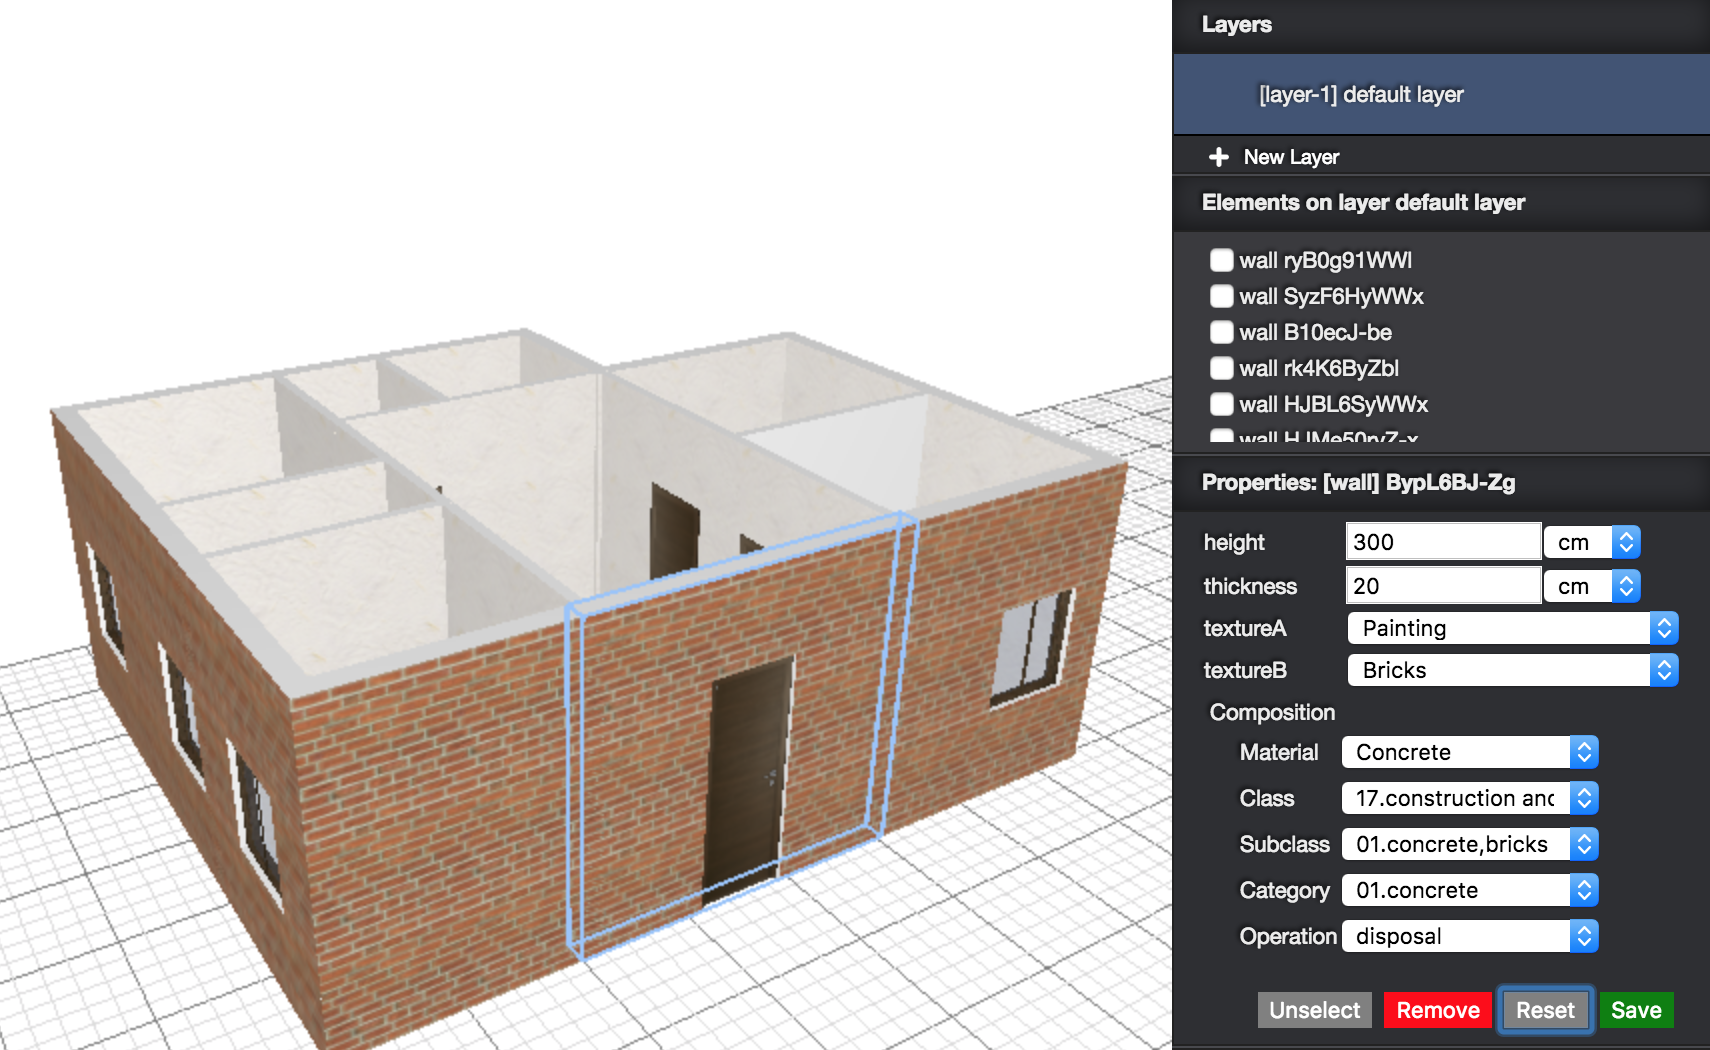
\includegraphics[width=1\linewidth]{images/3d-sel.png}
  \caption{Graphical interface for semantics annotation}
  \label{fig:semantics}
\end{figure}

\paragraph{Augmented reality visualization} 

\noindent
After modeling and attribution of semantics to components, the quantity surveyor can validate the entire model by spatial merging into a 3D point cloud (see Figure~\ref{fig:augmented}) previously obtained by using flying drones for the exterior, or 3D laser scanners for the interior. In this way one can assess the adhesion of the modeled building structure to reality, possibly retracing to some previous step if the result is still not satisfactory.

\begin{figure}[htbp] %  figure placement: here, top, bottom, or page
   \centering
   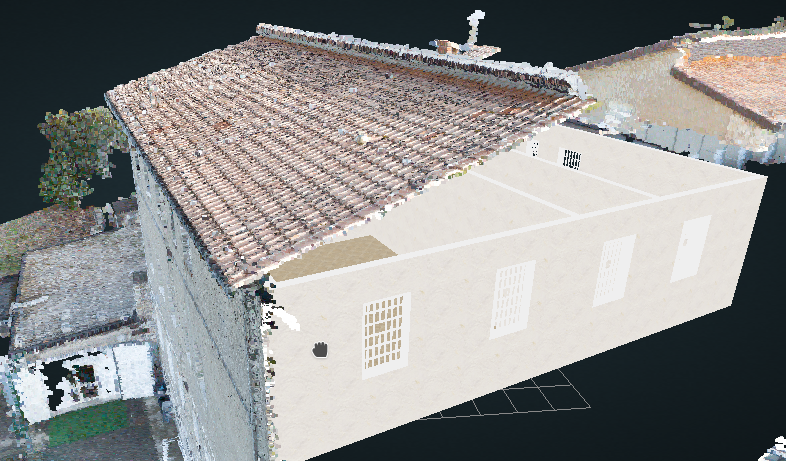
\includegraphics[width=1\linewidth]{images/augmented}
   \caption{A model inside a point cloud}
   \label{fig:augmented}
\end{figure}

\subsection{Process output}

\noindent 
Once the work is done and the model geometry is validated, the application provides a final report.
In particular, the final report will allow the quantity surveyor and/or the other professionals involved in the deconstruction design team, to determine whether the decision taken is convenient both economically and/or environmentally.

The final report consists of four documents.
(i)~\emph{An estimate of volumes and weights of materials}, computed by appropriate integration calculations, based on the geometry of components and annotations defined on them.
(ii)~\emph{An estimate of demolition costs}, including disposal and recovery.
Starting from volumes and densities of materials, and from EWC codes and hence the mode of disposal, it is estimated the cost of the contribution to landfills.
(iii)~\emph{The transportation costs} to move the materials to the closest landfills, taking into account the geographical position of the building, and by calculating the most convenient road routes.
(iv)~\emph{An estimate of the expected time} for the complete demolition of the building, located on a Gantt chart. Semantic annotations are also used to generate a schedule of the demolition activities by means of a PERT program.

%\section{\uppercase{Design and Architecture}}
\label{sec:architecture}

% principles
\noindent Workflow and requirements described in the previous section have been received in a prototypal application serving as proof of concept. With the aim of maximize accessibility for surveyors, it is strongly web based and runs in all modern browsers. It is built using React by Facebook and an MVC design pattern with \emph{unidirectional data flow} \cite{redux}:  it ensures the best code maintainability and debuggability by centralizing access to the application state to a single controller.

\vspace{-3mm}\subsection{UI \& UX}\vspace{-3mm}

The web application presents itself as a simplified CAD,  the UI comprises three main areas of interaction: \emph{toolbar}, \emph{canvas} and \emph{sidebar}, as shown by Figures~\ref{fig:ui} and~\ref{fig:ui2}.

\begin{figure}[htbp] %  figure placement: here, top, bottom, or page
   \centering
   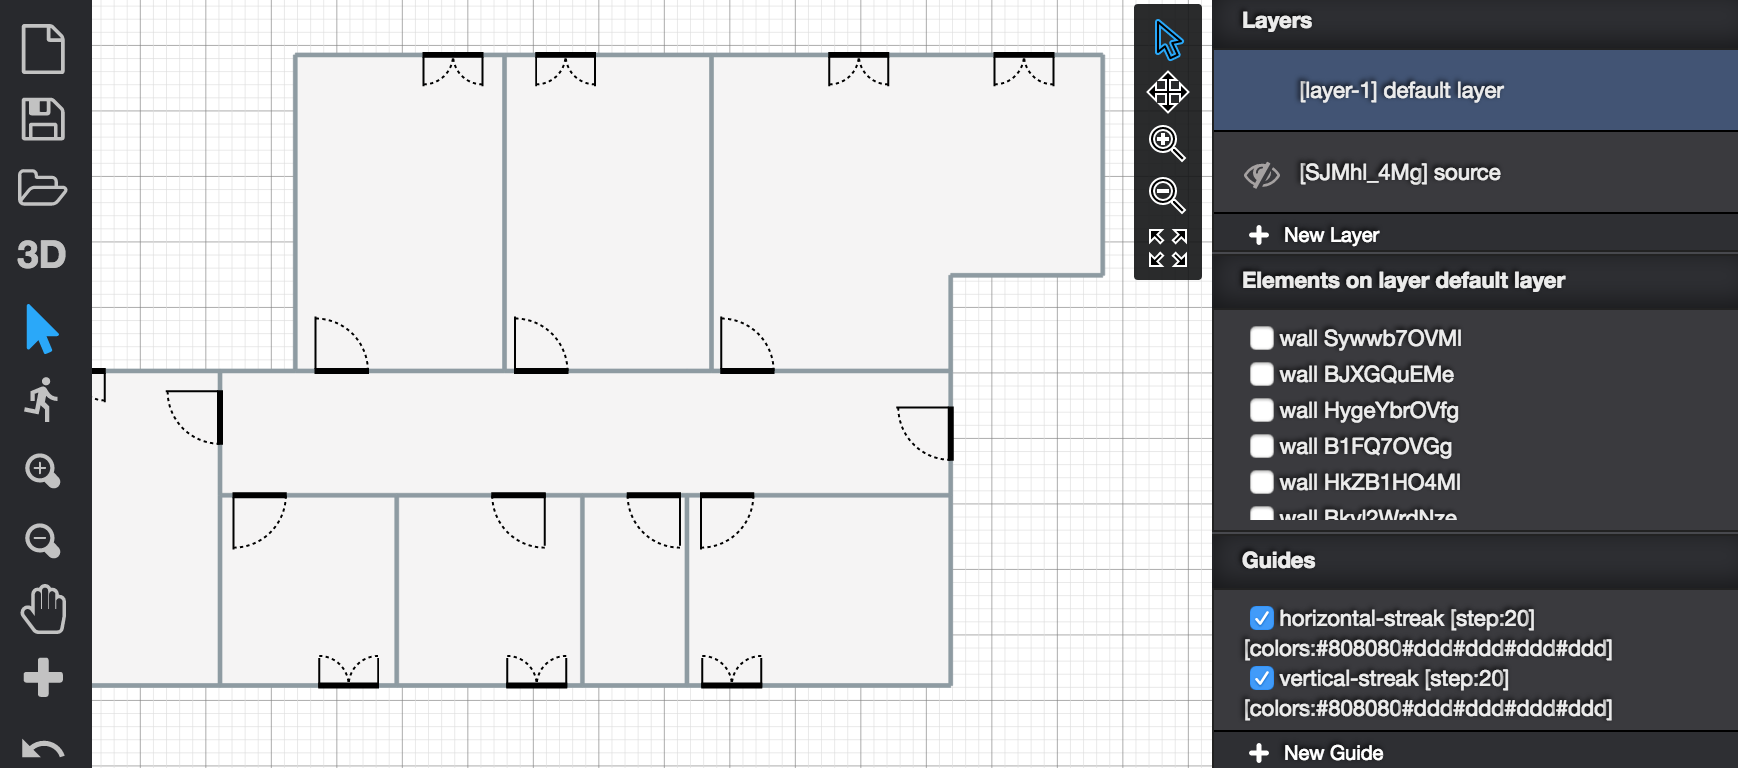
\includegraphics[width=1\linewidth]{images/2d}
   \label{fig:ui}
   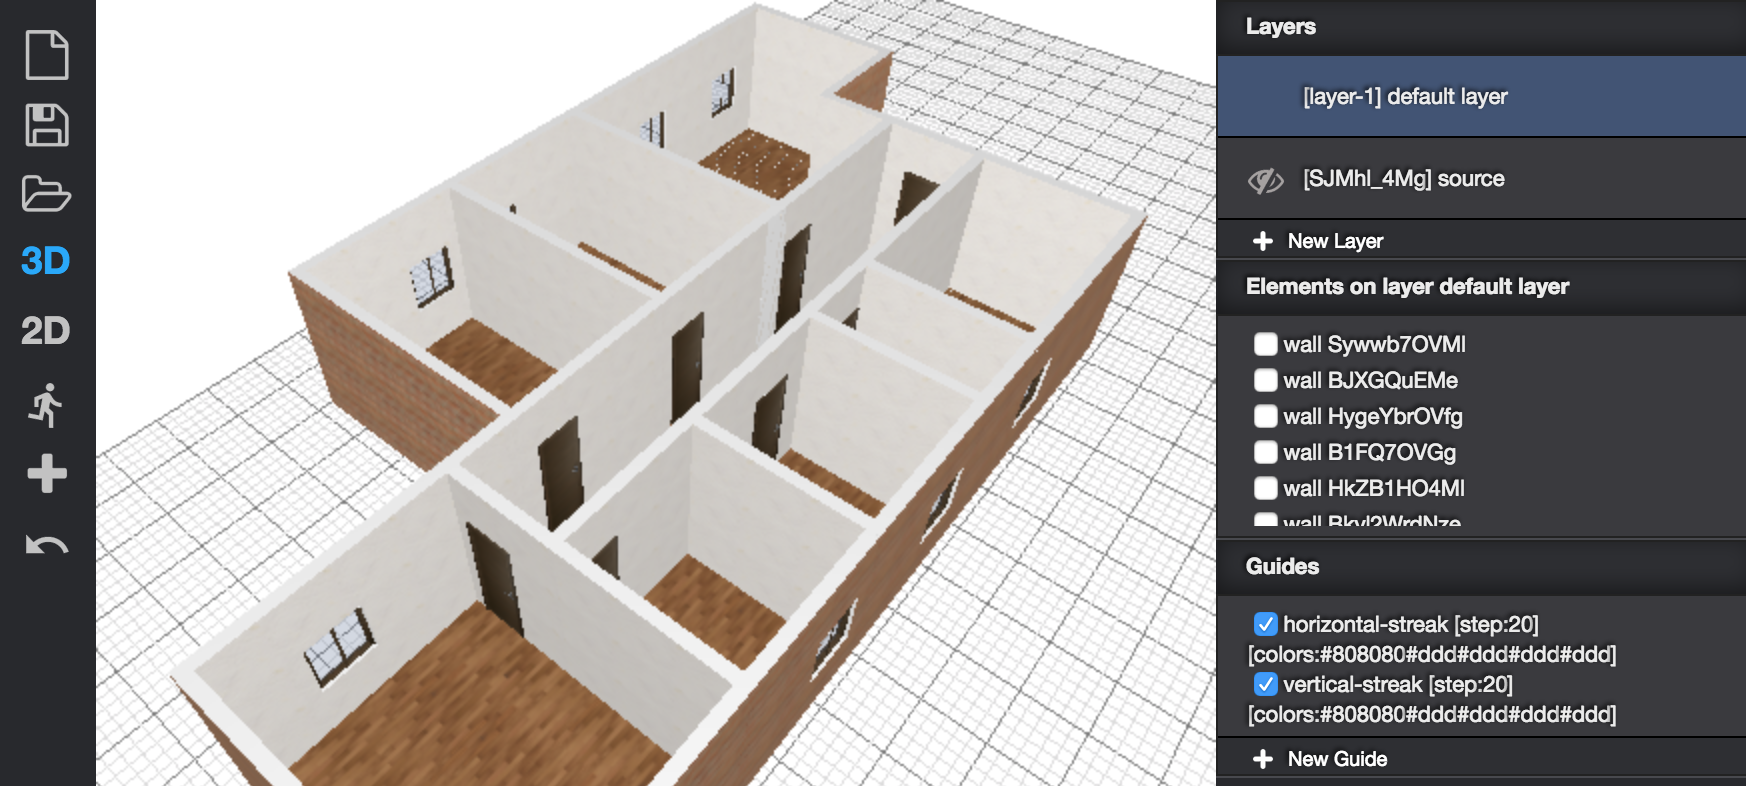
\includegraphics[width=1\linewidth]{images/3d}
   \caption{\emph{Metior} user interface: (a) 3D canvas; (b) 3D canvas}
   \label{fig:ui2}
\end{figure}

From the \emph{toolbar} the user can access functionalities related to: (1) project life cycle ({\tt new}, {\tt save}, {\tt load}); (2) project editing  ({\tt  show-catalog}); (3) view/interaction mode switching ({\tt 2D}, {\tt  3D}); interaction mode changing ({\tt  selecting}, {\tt pan}, {\tt zoom}).


The \emph{canvas} is the area in which the user can interact with actual model data. It supports two different view and interaction modes: (1) in~\emph{2D-mode} the model is displayed as a 2D projection from the top, and the interaction consists of element insertion, selection and editing (according to specific plugin interaction prototype, see~\ref{ssec:taxonomy}); (2) in~\emph{3D-mode} a 3D model can be inspected and navigated, respectively via trackball or first-person interaction style, while object picking allows for element selection.

The \emph{sidebar} shows the properties of the currently selected element.
In the properties panel it is possible to view the description of the element, to add/remove metadata, and to modify any property. The latter is the interaction mode that allows the user to associate semantics annotations to every part of the model.

\vspace{-3mm}\subsection{Plugin-architecture}\vspace{-3mm}

\noindent The application has been designed to provide a small set of core interaction functionalities and to encapsulate the generation logic for architectural components (from the very basic to the most articulated) into specific plugins.

A \emph{plugin} is a software component that can be seamlessly integrated into the system in order to extends its capabilities.
In \emph{Metior}, a plugin represents an architectural element that extends the Building Information Model design.
Technically, a plugin represents a \emph{prototype} (namely a ``class'' in OOP) of a construction element that can be inserted (``instantiated'') into the \emph{canvas}, thus defining a new element, i.e. a new component of the model.

\subsubsection{Plugin definition}

A plugin is described by the following eight properties: (1) a unique name; (2) a description; (3) a set of metadata; (4) the \emph{occupation type} (one among \emph{linear}, \emph{area} or \emph{volume}); (5) the \emph{placement type} (\emph{inside} or \emph{over}); (6) a set of specific properties mapping the semantic to associate to the plugin; (7) a construction function that returns the 2D representation of the element in SVG format, to be used in the \emph{2D-mode}; (8) a construction function that returns the 3D representation of the element in OBJ format, to be used in the \emph{3D-mode}.

\subsubsection{Plugins taxonomy}\label{ssec:taxonomy}

\noindent The plugins can be organized according to the \emph{occupation type} and the \emph{placement type}. 

In the \emph{occupation type} three different kind of plugins can be identified: \emph{linear}, \emph{area} or \emph{volume} plugins.
The \emph{linear} ones extend in one dimension (unless a radial thickness) (e.g. hydraulic lines, electrical cables). The \emph{area} plugins extend in two dimensions (unless a linear thickness), (e.g. separation elements). They can be divided into \emph{horizontal area} (e.g. floor and ceil), and \emph{vertical area}, (e.g. walls). The \emph{volume} plugins extend in three dimensions. They can be \emph{fixed volume}, (e.g. a piece of furniture) and \emph{scalable volume}, that can be scaled (proportionally or not), (eg. pillars, staircases).

The \emph{occupation type} determines a different way to instantiate and to insert the plugins into the canvas.
In particular, in \emph{2D-mode}, \emph{linear} plugins are inserted drawing lines by mean of a drag\&drop interaction;
the \emph{area} plugins are inserted drawing the bounding-box of the element by mean of a drag\&drop interaction;
the \emph{volume} plugins are inserted picking the position of the element by mean of a point\&click interaction,
and adjusting their dimensions modifying the bounding-box by drag\&drop.

The \emph{placement type} determines if the element can be inserted into the canvas in a specific point occupied or not by other elements. In other words 
the {placement type} determines the relationship between a new instance of a plugin and instances of other plugins previously added to the model. The relationship can be of two kind: \emph{inside} or \emph{over}.
Plugins belonging to the \emph{inside} category can be added only inside other element (that can be \emph{linear}, \emph{area} or \emph{volume}); e.g., a ``window'' is a ``volume inside vertical area'' element,
while an ``hydraulic line'' is a ``linear inside horizontal area'' element.
Plugins of the \emph{over} category can be added only over other elements (of any type);
e.g., a ``pillar'' is a ``volume over horizontal area'' element,
while an ``electric panel'' is a ``volume over vertical area'' element.

In the design phase, an element that doesn't meet the placement constraints defined by the \emph{placement type} is notified by the system as a visual warning, showing its bounding-box in semi-transparent blinked red color.

\begin{figure}[htbp] %  figure placement: here, top, bottom, or page
   \centering

   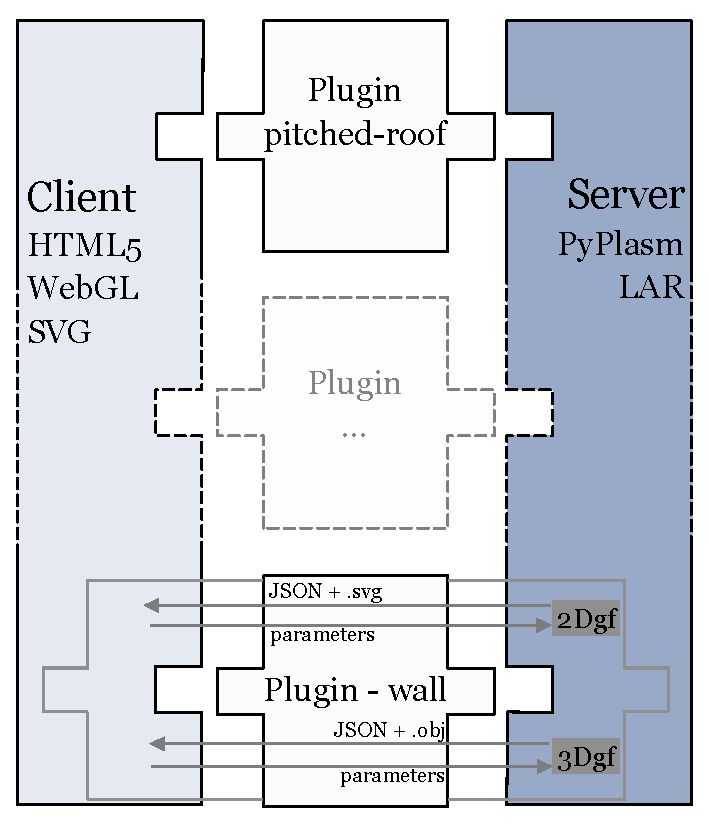
\includegraphics[width=0.6\linewidth]{images/architecture-h}

   \caption{Client/Server architecture for server-side model generation.}
   \label{fig:c-s-arch}
\end{figure}

\subsubsection{Plugin specific properties}

\noindent Each plugin has a set of specific properties of the building elements it represents.
Each property is defined by a  \emph{name}, a \emph{type}, such as ``number'', ``text'', ``boolean'', or ``custom'', and by a \emph{value}.
According to its type, each property value can be inserted in different ways.
For example, a boolean property value is set through a checkbox, while a textual property is set through a text box.

The system is designed to accept custom kinds of property. A custom property is required to define the component of the UI that permit the user to insert its value.
For example, a ``color'' property can be introduced by defining a UI component composed by three text boxes (one for each RGB components), while a ``length'' property can be introduced by defining a UI component including a text box for the value and a drop-down menu for the unit of measure.

The specific properties of an element can be edited in the relative panel in the sidebar, once the element is selected in the canvas.

\vspace{-3mm}\subsection{Plugin Catalog}\vspace{-3mm}
\noindent It is pivotal to provide surveyors with a rich catalog of plugins, to cover all the basic as well as the most advanced modeling requirements. Table~\ref{tab:plugins-example} reports examples of plugins arranged according to the  taxonomy introduced in Section~\ref{ssec:taxonomy}.

\begin{table}[htbp]
\small
\centering
\caption{Plugin examples according to taxonomy}
\begin{tabular}{|
>{\columncolor[HTML]{EFEFEF}}l |l|l|}
\hline
{\color[HTML]{000000} } & \cellcolor[HTML]{EFEFEF}{\color[HTML]{000000} \footnotesize{\bf{inside}}} & \cellcolor[HTML]{EFEFEF}{\color[HTML]{000000} \footnotesize{\bf{over / free}}} \\ \hline
\footnotesize{\bf{linear}}      & \tt{pipe}             & \tt{electrical-conduit}  \\ \hline
\footnotesize{\bf{ver. area}}   & \tt{window, door}     & \tt{wall}                \\ \hline
\footnotesize{\bf{hor. area}}   & \tt{light-panel}      & \tt{ground, ceil}        \\ \hline
\footnotesize{\bf{volume}}      & \tt{pillar}           & \tt{staircase}           \\ \hline
\end{tabular}
\label{tab:plugins-example}
\end{table}


\vspace{-3mm}\subsection{Server-side models generation}\vspace{-3mm}

\noindent Both the 3D and 2D model generations have been designed as \emph{asynchronous}. The actual result of the invocation of a generating function is not the generated model itself, but rather a \emph{promise} of the expected result. Such a design choice is important since the computation for model generation may require some while. In the meantime the user must be able to interact with the interface, which in turn must remain responsive. Relying on this architecture, generation of the models can be easily delegated to a server (as shown in Figure~\ref{fig:c-s-arch}), thus relieving the client from the burden of onerous computations. The server exposes a REST-like HTTP-based JSON API to the client. The plugins span from the client to the server, since the 2D and 3D generating functions  defined by the plugin, with superclasses \emph{2Dgf} and \emph{3Dgf}, are actually executed on the server, as shown in Figure~\ref{fig:c-s-arch} .


\vspace{-1mm}\subsection{Plugin example}\vspace{-3mm}

In Figure~\ref{spiralstair} is shown the plugin used to generate a spiral concrete frame, where the steps are obtained by coded update of the polyhedral approximation of \texttt{larSolidHelicoid}, with parametric minor and major radiuses (\texttt{r} and \texttt{R}) and int number of \texttt{steps}. The \texttt{nturns} float is in radians.

\begin{figure}[h] %  figure placement: here, top, bottom, or page
   \centering
   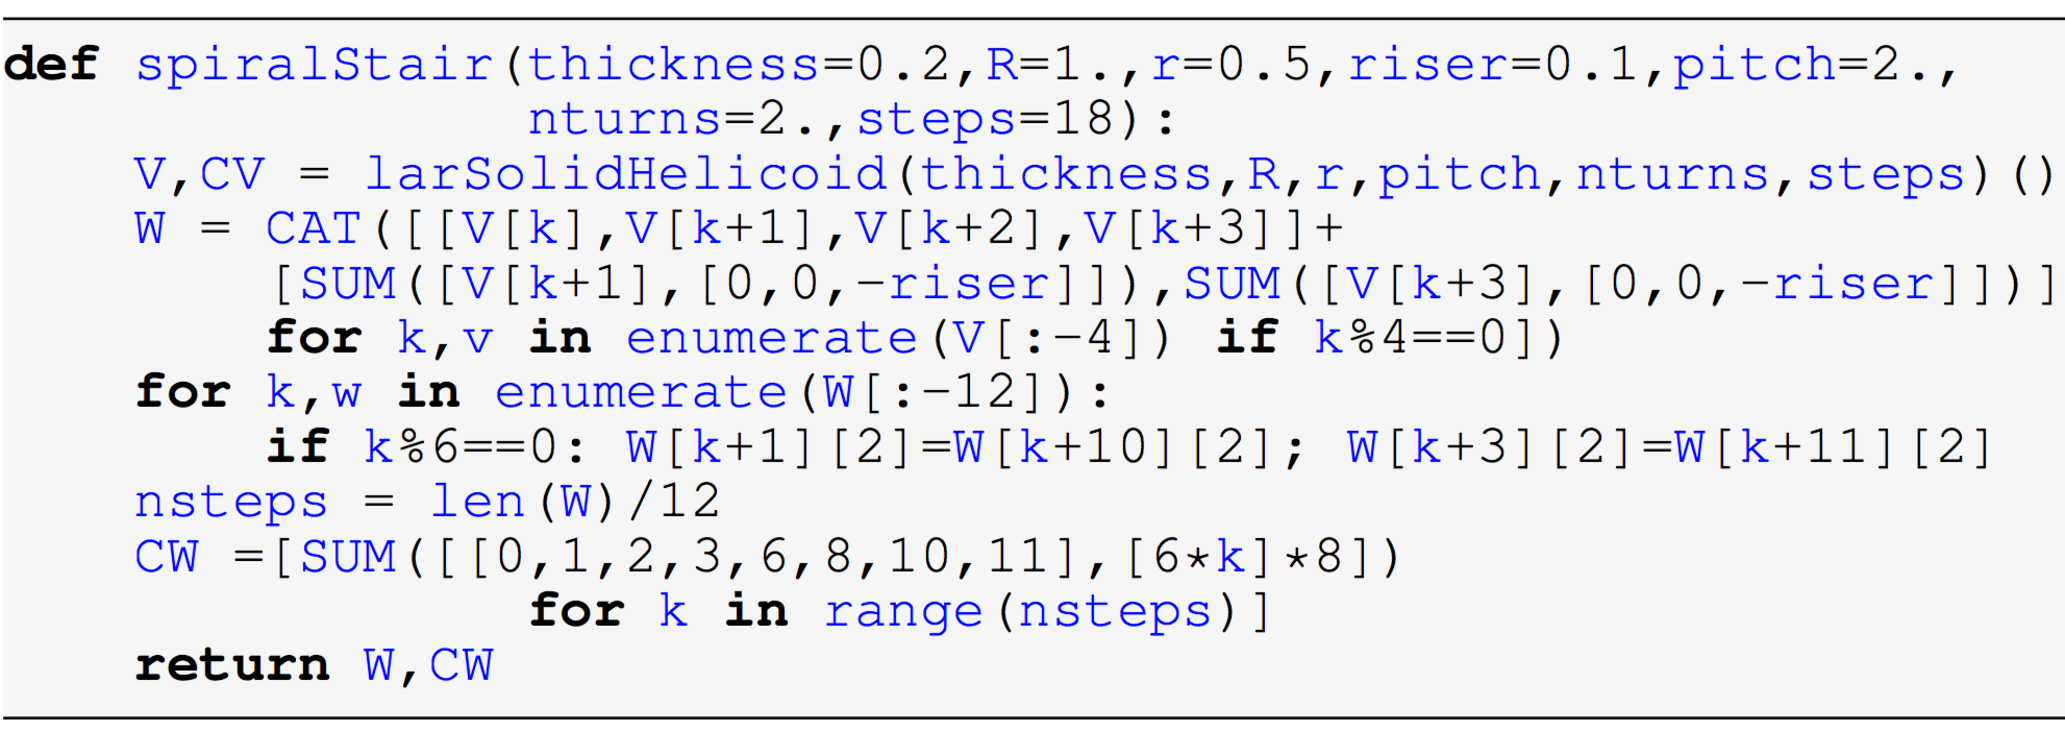
\includegraphics[width=\linewidth]{images/spiralstair}
   
   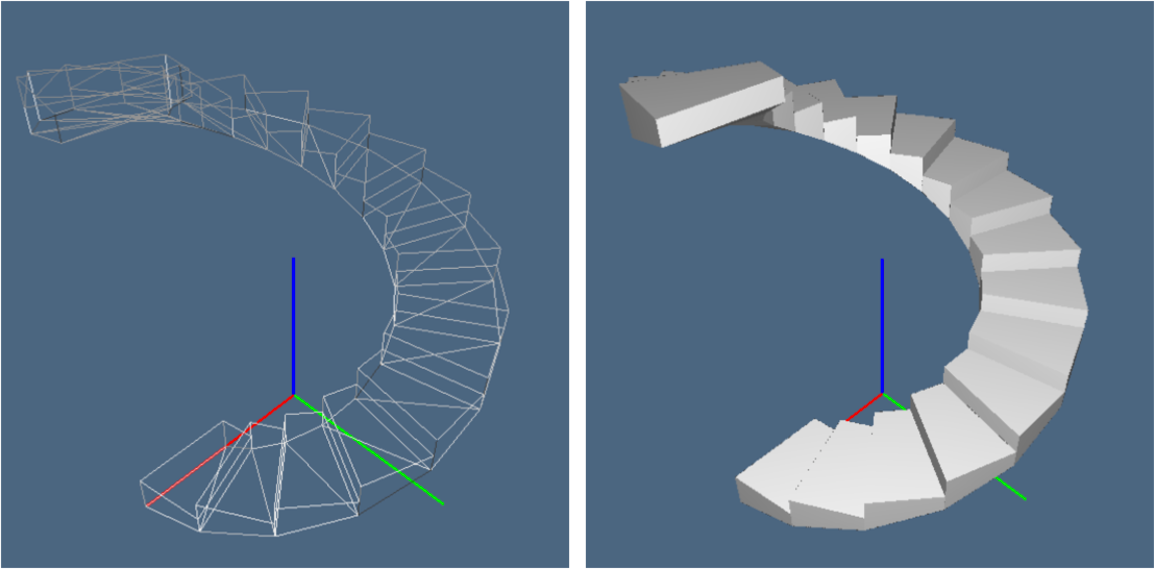
\includegraphics[width=\linewidth]{images/spiralstair2}
   \caption{(a) The generating function of a strongly parameterized \texttt{spiralStair}; (b) default \texttt{spiralStair}.}
   \label{spiralstair}
\end{figure}


\section{\uppercase{Design and Architecture}}
\label{sec:architecture}

% principles

\noindent
Workflow and requirements described in the previous section have been received in a prototypal application serving as proof of concept. With the aim of maximize accessibility for quantity surveyors, it is strongly web based and runs in all modern browsers. It is built using React by Facebook and the \emph{unidirectional data flow} design pattern~\cite{redux}:  it ensures the best code maintainability and debuggability by centralizing access to the application state in a single controller.

\subsection{UI and user experience}

\noindent
The web application presents itself as a simplified CAD software, where the user interface comprises three main areas of interaction: \emph{toolbar}, \emph{canvas} and \emph{sidebar}, as shown by Figures~\ref{fig:ui2d} and~\ref{fig:ui3d}.

\begin{figure}[htbp] %  figure placement: here, top, bottom, or page
   \centering
   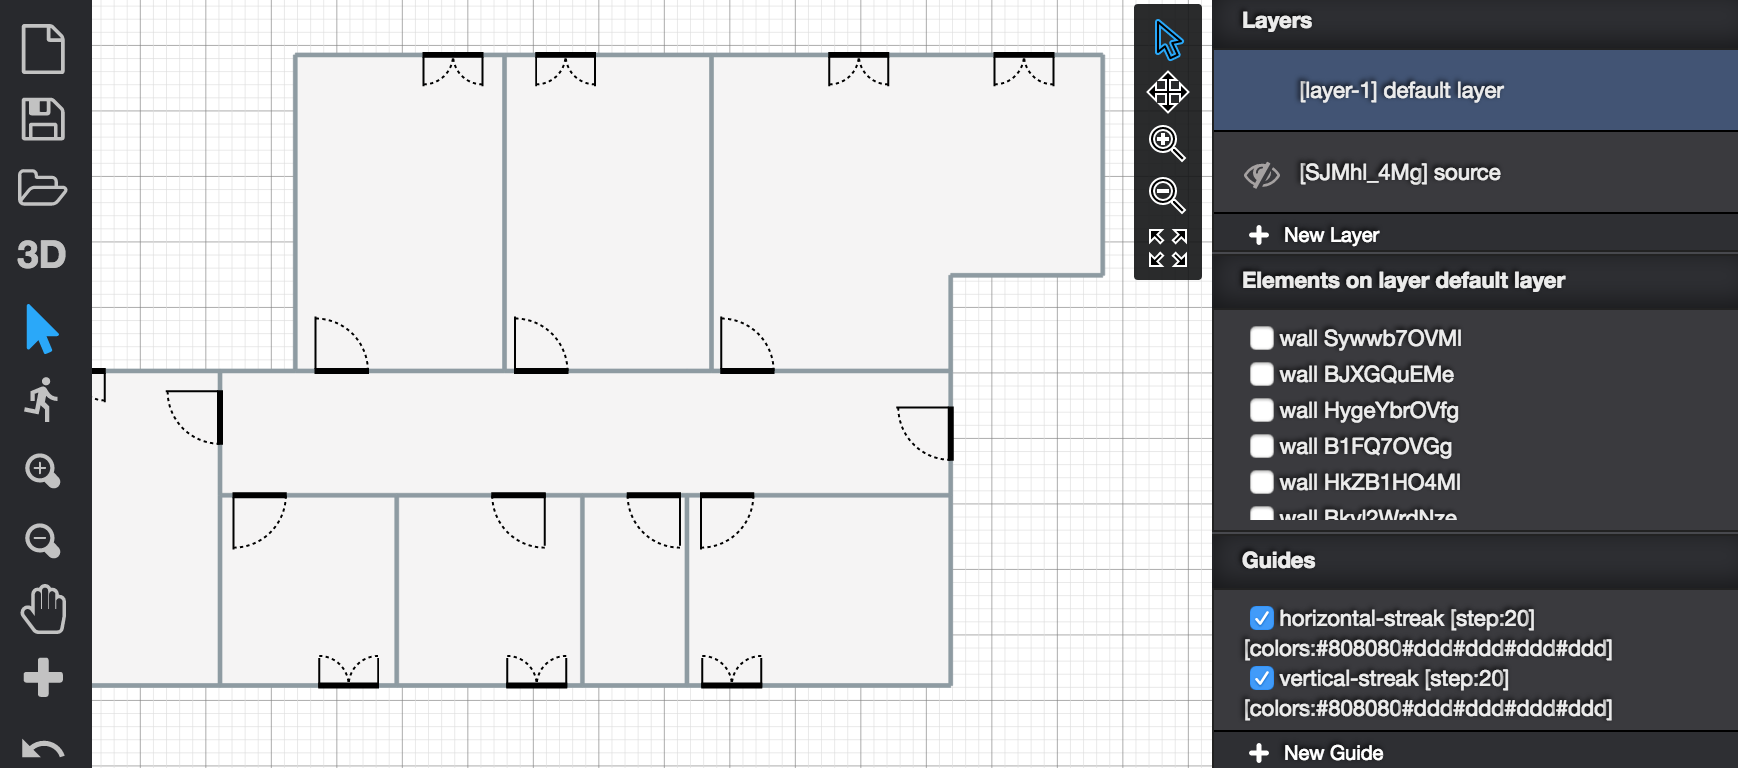
\includegraphics[width=1\linewidth]{images/2d}
   \caption{\emph{Metior} user interface: 2D canvas.}
   \label{fig:ui2d}
\end{figure}

\begin{figure}[htbp]
   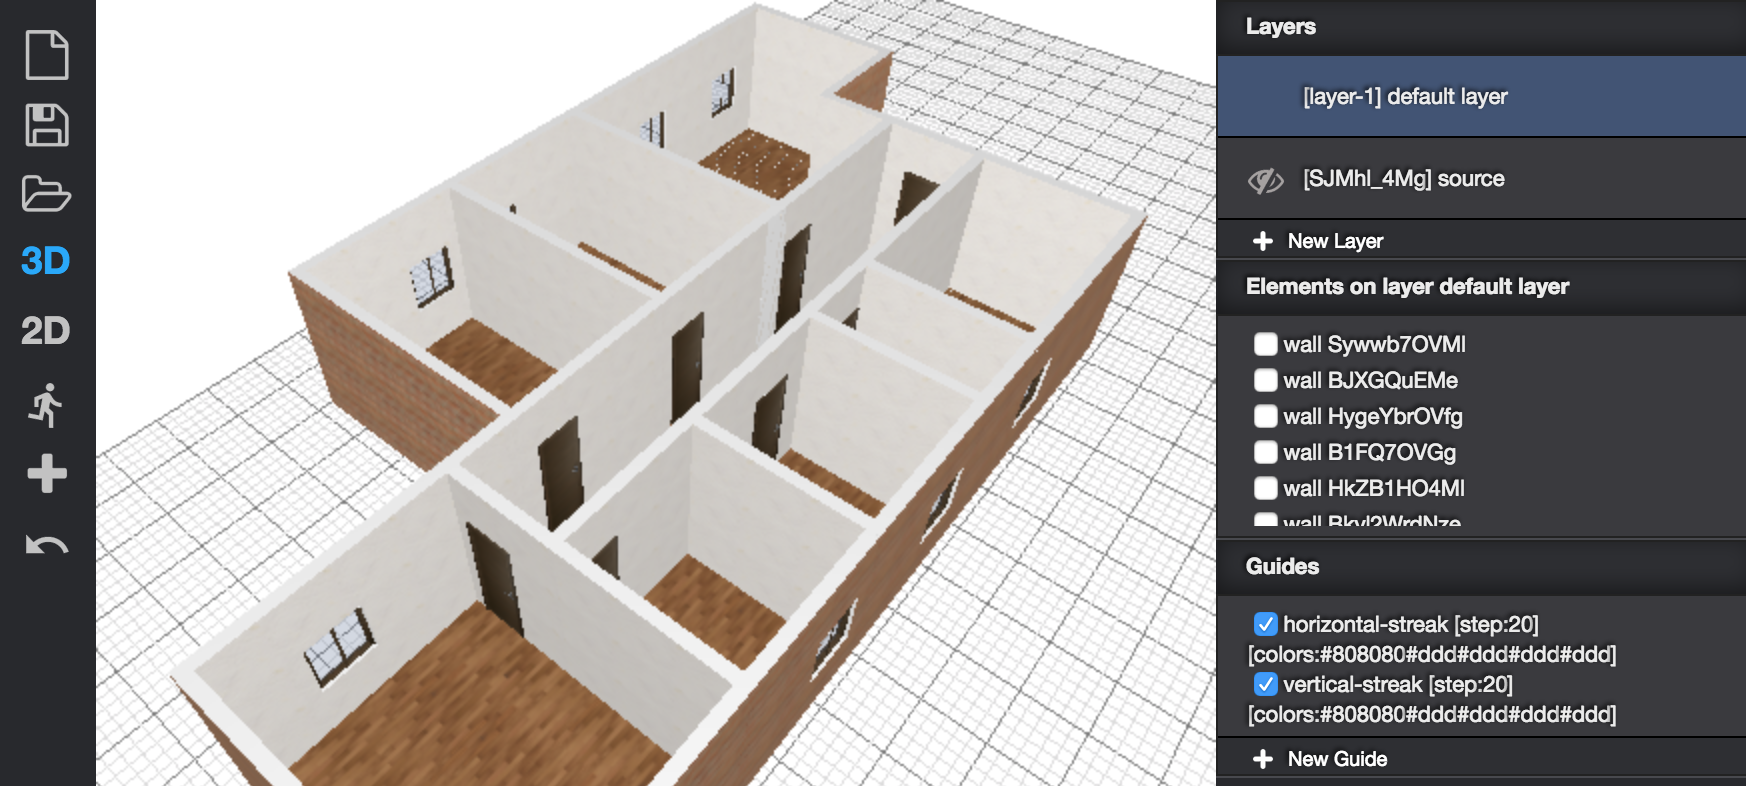
\includegraphics[width=1\linewidth]{images/3d}
   \caption{\emph{Metior} user interface: 3D canvas.}
   \label{fig:ui3d}
\end{figure}

From the \emph{toolbar} the user can access functionalities related to: project life cycle ({\tt new}, {\tt save}, {\tt load}); project editing  ({\tt  show-catalog}); view/interaction mode switching ({\tt 2D}, {\tt  3D}); interaction mode changing ({\tt  selecting}, {\tt pan}, {\tt zoom}).


The \emph{canvas} is the area in which the user can interact with actual model data. It supports two different views and interaction modes. In~\emph{2D-mode} the model is displayed as a 2D projection from the top, and the interaction consists of element insertion, selection and editing (according to specific plugin interaction prototype, see Section~\ref{ssec:taxonomy}). In~\emph{3D-mode} a 3D model can be inspected and navigated, respectively via trackball or first-person interaction style, while object picking allows for element selection.

The \emph{sidebar} shows the properties of the currently selected element.
In the properties panel it is possible to view the description of the element, to add/remove metadata, and to modify any property. The latter is the interaction mode that allows the user to associate semantic annotations to every part of the model.

\subsection{Plugin-architecture}

\noindent
The application has been designed to provide a small set of core interaction functionalities and to encapsulate the generation logic for architectural components (from the very basic to the most articulated) into specific plugins.

A \emph{plugin} is a software component that can be seamlessly integrated into the system in order to extends its capabilities.
In \emph{Metior}, a plugin represents an architectural element that extends the Building Information Model design.
Technically, a plugin represents a \emph{prototype} (namely a ``class'' in Object Oriented Programming) of a construction element that can be inserted (``instantiated'') into the \emph{canvas}, thus defining a new \emph{element}, i.e. a new component of the model.

\paragraph{Plugin definition}

\noindent
A plugin is described by the following eight properties: (1) a unique name; (2) a description; (3) a set of metadata; (4) the \emph{occupation type} (one among \emph{linear}, \emph{area} or \emph{volume}); (5) the \emph{placement type} (\emph{inside} or \emph{over}); (6) a set of specific properties mapping the semantic to associate to the plugin; (7) a \emph{generating function} that returns the 2D representation of the element in SVG format, to be used in the \emph{2D-mode}; (8) a \emph{generating function} that returns the 3D representation of the element in OBJ format, to be used in the \emph{3D-mode}.

\paragraph{Plugins taxonomy}
\label{ssec:taxonomy}

\noindent
The plugins can be organized according to \emph{occupation type} and \emph{placement type}.

In the \emph{occupation type} three different kind of plugins can be identified: \emph{linear}, \emph{area} or \emph{volume} plugins.
The \emph{linear} ones extend in one dimension (unless a radial thickness) (e.g. hydraulic lines, electrical cables). The \emph{area} plugins extend in two dimensions (unless a linear thickness), (e.g. separation elements). They can be divided into \emph{horizontal area} (e.g. floor and ceil), and \emph{vertical area}, (e.g. walls). The \emph{volume} plugins extend in three dimensions. They can be \emph{fixed volume}, (e.g. a piece of furniture) and \emph{scalable volume}, that can be scaled (proportionally or not), (eg. pillars, staircases).

The \emph{occupation type} determines a different way to instantiate and to insert the plugins into the canvas.
In particular, in \emph{2D-mode}, \emph{linear} plugins are inserted drawing lines by mean of a drag\&drop interaction;
the \emph{area} plugins are inserted drawing the bounding-box of the element by mean of a drag\&drop interaction;
the \emph{volume} plugins are inserted picking the position of the element by mean of a point\&click interaction,
and adjusting their dimensions modifying the bounding-box by drag\&drop.

\begin{table}[tbp]
\small
\centering
\caption{Plugin examples according to taxonomy}
\begin{tabular}{|
>{\columncolor[HTML]{EFEFEF}}l |l|l|}
\hline
{\color[HTML]{000000} } & \cellcolor[HTML]{EFEFEF}{\color[HTML]{000000} \footnotesize{\bf{inside}}} & \cellcolor[HTML]{EFEFEF}{\color[HTML]{000000} \footnotesize{\bf{over / free}}} \\ \hline
\footnotesize{\bf{linear}}      & \tt{pipe}             & \tt{electrical-conduit}  \\ \hline
\footnotesize{\bf{ver. area}}   & \tt{window, door}     & \tt{wall}                \\ \hline
\footnotesize{\bf{hor. area}}   & \tt{light-panel}      & \tt{ground, ceil}        \\ \hline
\footnotesize{\bf{volume}}      & \tt{pillar}           & \tt{staircase}           \\ \hline
\end{tabular}
\label{tab:plugins-example}
\end{table}

The \emph{placement type} determines if the element can be inserted into the canvas in a specific point occupied or not by other elements. In other words, the {placement type} determines the relationship between a new instance of a plugin and instances of other plugins previously added to the model. The relationship can be of two kind: \emph{inside} or \emph{over}.
Plugins belonging to the \emph{inside} category can be added only inside other element (that can be \emph{linear}, \emph{area} or \emph{volume}); e.g., a ``window'' is a ``volume inside vertical area'' element,
while an ``hydraulic line'' is a ``linear inside horizontal area'' element.
Plugins of the \emph{over} category can be added only over other elements (of any type);
e.g., a ``pillar'' is a ``volume over horizontal area'' element,
while an ``electric panel'' is a ``volume over vertical area'' element.

In the design phase, an element that doesn't meet the placement constraints defined by the \emph{placement type} is notified by the system as a visual warning, showing its bounding-box in semi-transparent blinked red color.

\begin{figure}[htbp] %  figure placement: here, top, bottom, or page
   \centering

   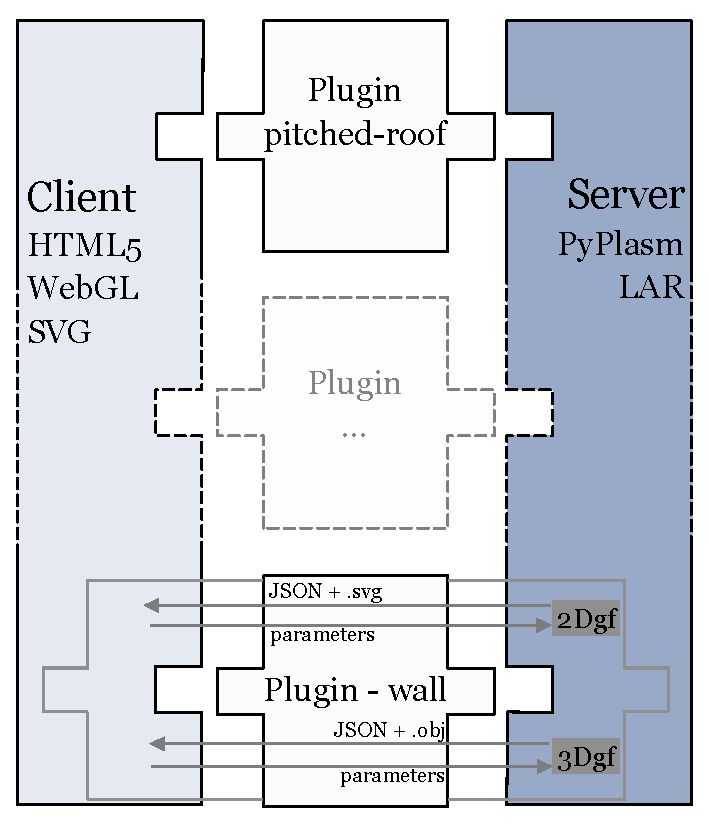
\includegraphics[width=0.6\linewidth]{images/architecture-h}

   \caption{Client/Server architecture for server-side model generation.}
   \label{fig:c-s-arch}
\end{figure}

\paragraph{Plugin specific properties}

\noindent
Each plugin has a set of specific properties of the building elements it represents.
Each property is defined by (1) a \emph{name}, (2) a \emph{type}, such as ``number'', ``text'', ``boolean'', or ``custom'', and by  (3) a \emph{value}.
According to its type, each property value can be inserted in different ways.
For example, a boolean property value is set through a checkbox, while a textual property is set through a text box.

The system is designed to accept custom kinds of property. A custom property is required to define the component of the UI that permits the user to insert its value.
For example, a ``color'' property can be introduced by defining a UI component composed by three text boxes (one for each RGB components), while a ``length'' property can be introduced by defining a UI component including a text box for the value and a drop-down menu for the unit of measure.

The specific properties of an element can be edited in the relative panel in the sidebar, once the element is selected in the canvas.

\subsection{Plugin Catalog}

\noindent
It is pivotal to provide the system users with a rich catalog of plugins, to cover all the basic as well as the most advanced modeling requirements. Table~\ref{tab:plugins-example} reports examples of plugins arranged according to the  taxonomy introduced in Section~\ref{ssec:taxonomy}.

\subsection{Server-side models generation}

\noindent
Both the 3D and 2D model generations have been designed as \emph{asynchronous}. The actual result of the invocation of a generating function is not the generated model itself, but rather a \emph{promise} of the expected result. Such a design choice is important since the computation for model generation may require some while. In the meantime the user must be able to interact with the interface, which in turn must remain responsive. Relying on this architecture, generation of the models can be easily delegated to a server (as shown in Figure~\ref{fig:c-s-arch}), thus relieving the client from the burden of onerous computations. The server exposes a REST-like HTTP-based JSON API to the client. The plugins span from the client to the server, since the 2D and 3D generating functions ( \emph{2Dgf} and \emph{3Dgf}) defined by the plugin are actually executed on the server, as shown in Figure~\ref{fig:c-s-arch}.

\subsection{Plugin examples}

\begin{figure}[hbt] %  figure placement: here, top, bottom, or page
   \centering
   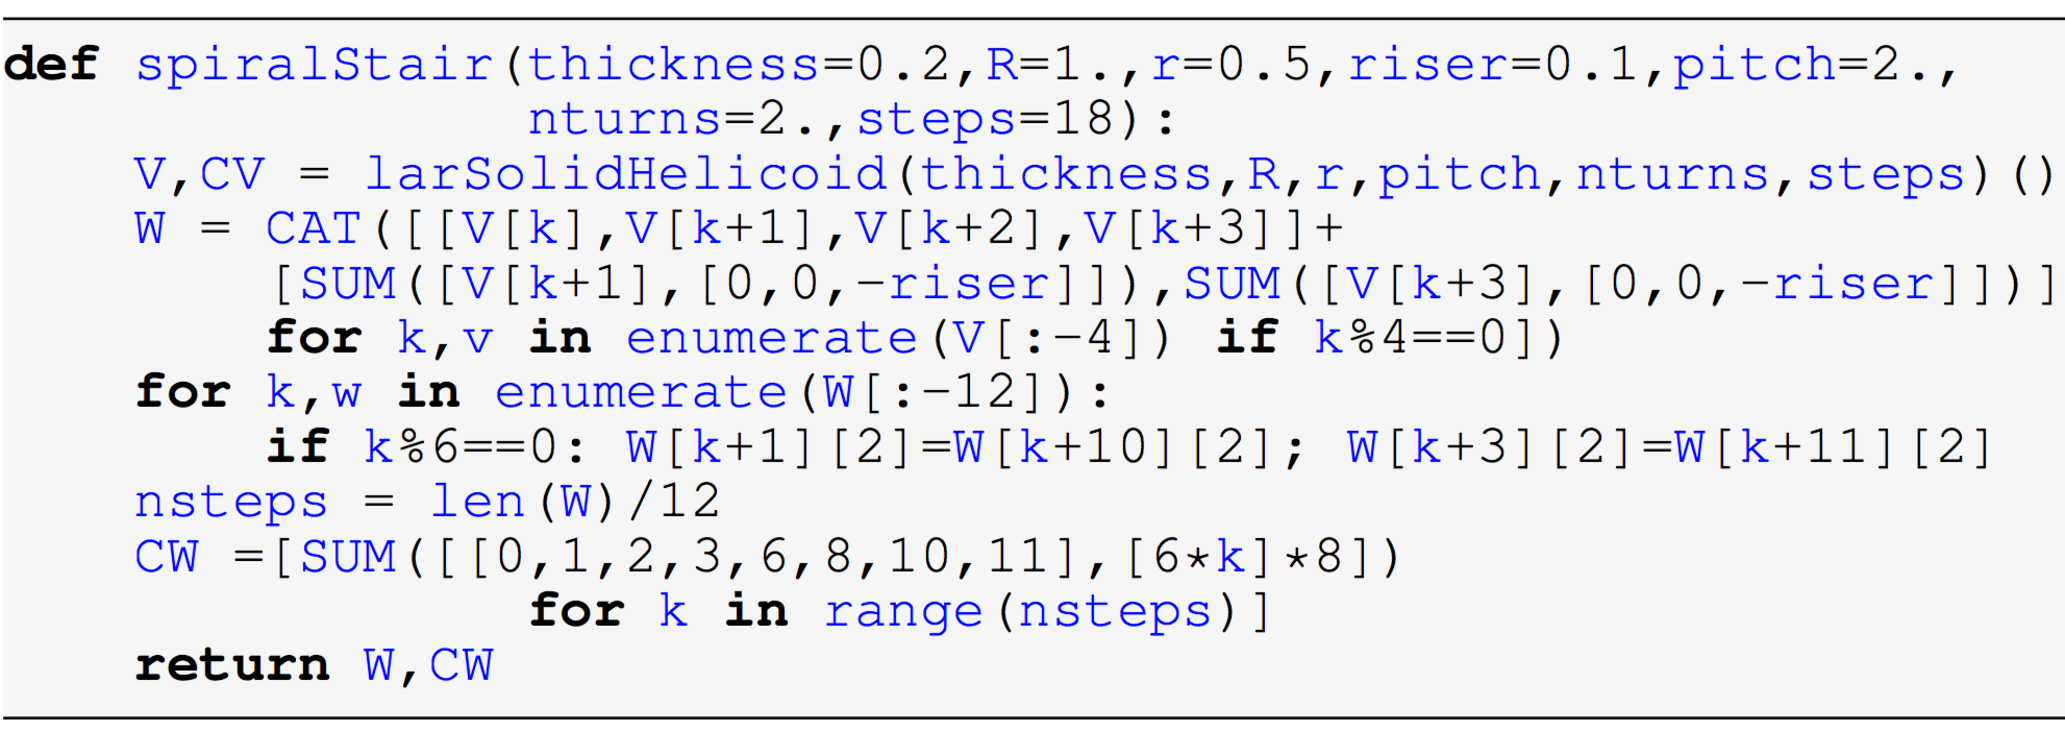
\includegraphics[width=\linewidth]{images/spiralstair}
   
   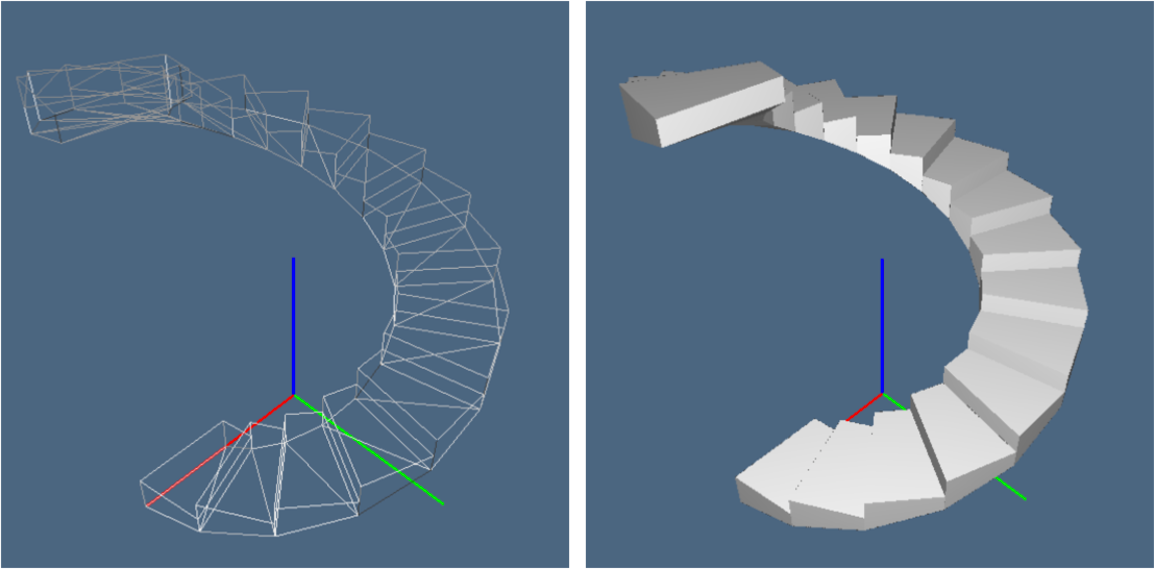
\includegraphics[width=\linewidth]{images/spiralstair2}
   \caption{(a) The generating function of a strongly parameterized \texttt{spiralStair}; (b) default \texttt{spiralStair}.}
   \label{spiralstair}
\end{figure}

\noindent
Figure~\ref{spiralstair} shows the plugin used to generate concrete spiral stairs, with steps from coded update of a polyhedral approximation of a \texttt{larSolidHelicoid()},  minor and major radiuses (\texttt{r} and \texttt{R}) and \texttt{int} number of \texttt{steps}. The \texttt{nturns} float is in radians. 

The model generated by a plugin for automatic generation of spatial concrete frames is shown in Figure~\ref{spatialFrame}. In this case the user interface produces a small \texttt{.csv} file specifying, for each component \emph{planar frame}, the grid-like pattern of members, the 2D sections of columns and beams, and the proper roto-translation, i.e.~the four numbers $\alpha, tx, ty, tz$ that instantiate each frame in the reference frame of the previous one. The connecting beams are automatically generated, and the various classes of members (\texttt{foots,timbers,columns,linkBeams}) are made available for interactive picking and possible local modification of geometry and/or materials by the system user, and of course, for quantity surveying.


\begin{figure}[t] %  figure placement: here, top, bottom, or page
   \centering
   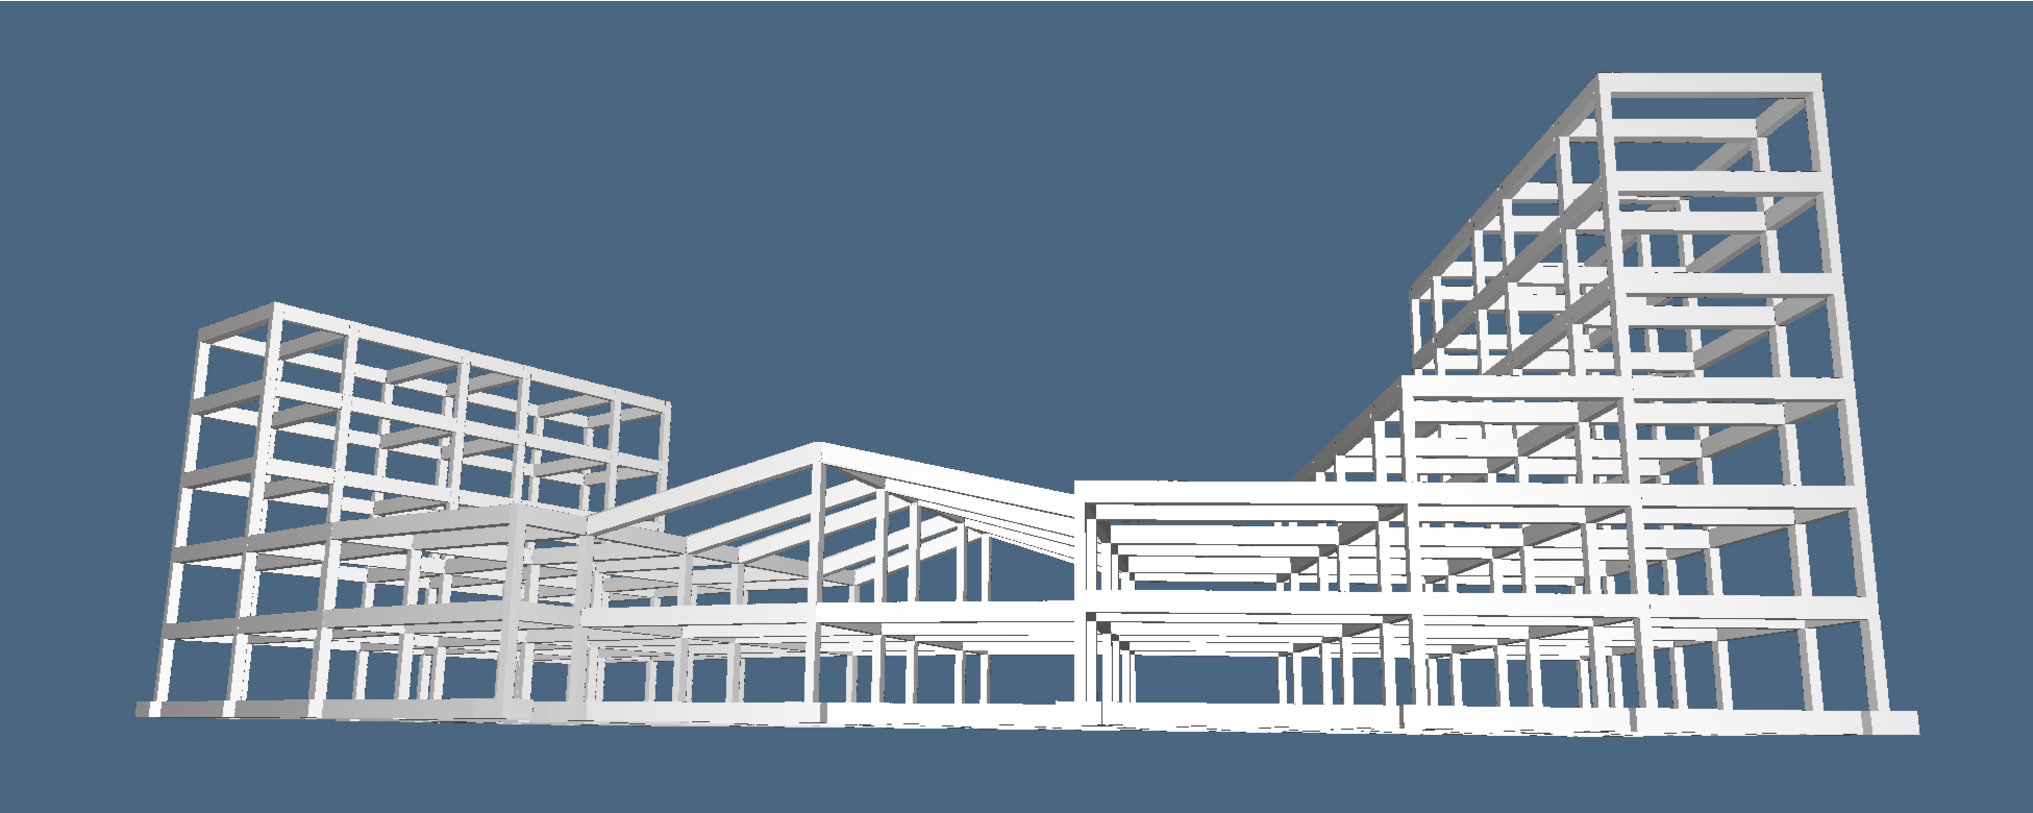
\includegraphics[width=\linewidth]{images/frame}
      \caption{A spatial concrete frame generated, from a small \texttt{.csv} file, by the \texttt{pyplasm} plugin \texttt{spatialFrame}.}
   \label{spatialFrame}
\end{figure}


%\section{\uppercase{Solid Modeling}}
\label{sec:modeling}

\noindent
The server-based geometric core of the modeling architecture is based on a set of python libraries, including \texttt{pyopengl}, \texttt{scipy}, \texttt{pyplasm} and \texttt{larlib}, that provide our current implementation of the LAR (Linear Algebraic Representation) scheme for solid modeling, 3D imaging and mesh representation, and which is briefly described in the following.

\vspace{-3mm}\subsection{Linear Algebraic Representation}\vspace{-3mm}

LAR is a general-purpose representation scheme~\cite{Dicarlo:2014:TNL:2543138.2543294} for geometric and solid modeling introduced recently. The domain of the scheme is provided by dimension-independent \emph{cellular complexes}, while its codomain is that of \emph{sparse matrices}, stored using either the CSR (Compressed Sparse Row) or the CSC (Compressed Sparse Column) \texttt{scipy}'s memory format. The LAR polyhedral domain coincides with complexes of connected $d$-cells, even non-convex and/or including any number of holes. 

The very general shape allowed for cells makes the LAR scheme notably appropriate for solid modeling of buildings and their components. E.g., the whole frontage of a construction can be described as a single 3-cell of its solid model. Also, the algebraic foundation of LAR allows not only for fast queries about incidence and adjacency of cells, but also to resolve---via fast SpMV computational kernels---the boundary extraction of any 3D subset of the building model. 

It is worth noting that LAR provides a direct management of all subsets of cells and their physical properties trough the linear spaces of \emph{chains} induced by the model partitioning, and their dual spaces of \emph{cochains}. The linear operators of \emph{boundary} and \emph{coboundary} between such linear spaces, suitably implemented by sparse matrices, directly provide, depending on the dimension of the mapped spaces, the discrete differential operators of \emph{gradient}, \emph{curl} and \emph{divergence}, while their product gives the \emph{Laplacian}~\cite{ieee-tase}.  

\vspace{-3mm}\subsection{Geometric computing of shape}\vspace{-3mm}

Our computational environment is strongly oriented towards the most general parametric modeling of component shapes of buildings. This attitude is produced by two Python libraries, that provide a dimension-independent algebraic calculus with shapes (\texttt{pyplasm}) and their representation in the LAR scheme (\texttt{larlib}). 

PLaSM~\cite{Paoluzzi:1995:GPP:212332.212349,Paoluzzi:2001:GPC:600092}, which stands for Programming Language for Solid Modeling, is a geometry-oriented extension of the Backus' FL language~\cite{backus:78,BWWLA89}.  PLaSM is a project developed in the nineties in the framework of the \emph{Building Technologies Project} (\emph{``PF Edilizia''}) of the Italian National Research Council. The \texttt{pyplasm} module (2006-) is the C++ porting of PLaSM to Python via SWIG wrapping, providing several operators for fast and concise functional computing of shapes.

On top of the Scipy/Pyplasm stack we started (2012), using literate programming methods, to build a set of software modules, named \texttt{larlib}, and using the LAR scheme. This library provides the computation of topological queries and physical properties of meshes and complexes, including integration of polynomials over the boundary of any chain of cells. For interactive visualization it relies on the \texttt{pyplasm} viewer, based on OpenGL.
A porting of the most engaging parts of \texttt{larlib} to \emph{Julia}, the last-generation programming language  for scientific computing~\cite{BEKS14} started very recently, with the purpose of taking advantage of the great computational efficiency and parallelism of Julia in more demanding applications. 

\vspace{-3mm}\subsection{Plugin server framework}\vspace{-3mm}

Our building deconstruction framework  has a web-based client-server architecture,  discussed in Section~\ref{sec:architecture}. 	\emph{Metior}, the web client application, is illustrated in Section~\ref{sec:application}. The server-side of the framework, discussed in this section, is a  plugin server written in Python, which capitalizes on the stack of geometric programming tools described above. 

The Metior user quickly develops a 3D hierarchical assembly of different parts of the building envelope, as well as the horizontal and vertical partitions, using very simple 2D drawing tools. The more geometrically complex parts of the construction are conversely set up by user picking from context-based boards of predefined plugin templates, that are Python scripts~(see Figure~\ref{spiralstair}) generating solids models which are interactively dimensioned, partly by using 2D drawing tools, partly by user's numeric input from keyboard. 

Of course, our list of \emph{plugin templates} embraces most of building parts that are not manageable for quick shape input via 2D interaction. In particular, the picking boards include templates for planar concrete frames, spatial building frames, building foundations, roofs and stairs of different types, attics and dormers, fireplaces and fitted wardrobes, shover cabins and sanitary equipments, doors and windows, etc.

It is worth noting that, by virtue of the great expressiveness of the PLaSM operators and its functional style of programming, using first-class curried functions and dimension-independent geometry, the development of a new plugin template is very easy even for non-experienced programmers, and usually requires a tiny amount of time and code, that may range between 4-8 hours, and between 10-100 lines of Python/pyplasm code. 

Two important points we would like to remark are the following: (a) the expressive power of a geometric language is greatly empowered by  currying, i.e.~by the technique of translating the evaluation of a function that takes multiple arguments (or a tuple of arguments) into evaluating a sequence of functions, each with a single argument; (b) Python/pyplasm are used even to teach geometric programming to K12 students~\cite{ncLab} (see \href{https://nclab.com/3d-gallery/}{\texttt{https://nclab.com/3d-gallery/}}). 

Most of plugin templates currently used by Metior were developed in class by students of the computer  graphics course taught by A.P., one of the authors (see \href{https://github.com/cvdlab-courses/ggpl/blob/master/slides.md}{\texttt{https://github.com/cvdlab-courses/ggpl/}})). 



\section{\uppercase{Solid Modeling}}
\label{sec:modeling}

\ifreview

\noindent
The server-based geometric core of the modeling architecture is based on a set of python libraries, including \texttt{pyopengl}, \texttt{scipy}, \texttt{pyplasm} and \texttt{larlib}, that provide the current implementation of the LAR (Linear Algebraic Representation) scheme for solid modeling, 3D imaging and mesh representation, and which is briefly described in the following.

\else

\noindent
The server-based geometric core of the modeling architecture is based on a set of python libraries, including \texttt{pyopengl}, \texttt{scipy}, \texttt{pyplasm} and \texttt{larlib}, that provide our current implementation of the LAR (Linear Algebraic Representation) scheme for solid modeling, 3D imaging and mesh representation, and which is briefly described in the following.

\fi

\subsection{Linear Algebraic Representation}

\noindent
LAR is a general-purpose representation scheme~\cite{Dicarlo:2014:TNL:2543138.2543294} for geometric and solid modeling introduced recently. The domain of the scheme is provided by dimension-independent \emph{cellular complexes}, while its codomain is that of \emph{sparse matrices}, stored using either the CSR (Compressed Sparse Row) or the CSC (Compressed Sparse Column) \texttt{scipy}'s memory format. The LAR polyhedral domain coincides with complexes of connected $d$-cells, even non-convex and/or including any number of holes. 

The very general shape allowed for cells makes the LAR scheme notably appropriate for solid modeling of buildings and their components. E.g., the whole frontage of a construction can be described as a single 3-cell of its solid model. Also, the algebraic foundation of LAR allows not only for fast queries about incidence and adjacency of cells, but also to resolve---via fast SpMV computational kernels---the boundary extraction of any 3D subset of the building model. 

It is worth noting that LAR provides a direct management of all subsets of cells and their physical properties trough the linear spaces of \emph{chains} induced by the model partitioning, and their dual spaces of \emph{cochains}. The linear operators of \emph{boundary} and \emph{coboundary} between such linear spaces, suitably implemented by sparse matrices, directly provide, depending on the dimension of the mapped spaces, the discrete differential operators of \emph{gradient}, \emph{curl} and \emph{divergence}, while their product gives the \emph{Laplacian}~\cite{ieee-tase}.  

\subsection{Geometric computing of shape}

\noindent
Our computational environment is strongly oriented towards the most general parametric modeling of component shapes of buildings. This attitude is produced by two Python libraries, that provide a dimension-independent algebraic calculus with shapes (\texttt{pyplasm}) and their representation in the LAR scheme (\texttt{larlib}). 

PLaSM~\cite{Paoluzzi:1995:GPP:212332.212349,Paoluzzi:2001:GPC:600092}, which stands for Programming Language for Solid Modeling, is a geometry-oriented extension of Backus' FL language~\cite{backus:78,BWWLA89}.  PLaSM is a project developed in the nineties in the framework of \emph{Building Technologies Project} (\emph{``PF Edilizia''}) of the Italian National Research Council. The \texttt{pyplasm} module (2006) is the C++ porting of PLaSM to Python via SWIG wrapping.

On top of the Scipy/Pyplasm stack we started (2012), using literate programming methods, to build a set of software modules, named \texttt{larlib}, and using the LAR scheme. This library supports  topological queries and physical properties of meshes and complexes, including integration of polynomials over the boundary of any chain of cells. For interactive visualization it relies on the \texttt{pyplasm} viewer, based on OpenGL.
A porting of the most engaging parts of \texttt{larlib} to \emph{Julia}, the last-generation programming language for scientific computing~\cite{BEKS14} started very recently, with the purpose of taking advantage of the great computational efficiency and parallelism of Julia in more demanding applications. 

\subsection{Plugin server framework}

\noindent
Our building deconstruction framework  has a web-based client-server architecture,  discussed in Section~\ref{sec:architecture}.  \emph{Metior}, the web client application, is illustrated in Section~\ref{sec:application}. The server-side of the framework, discussed in this section, is a  plugin server written in Python, which capitalizes on the stack of geometric programming tools described above. 

The Metior user quickly develops a 3D hierarchical assembly of different parts of the building envelope, as well as the horizontal and vertical partitions, using very simple 2D drawing tools. The more geometrically complex parts of the construction are conversely set up by user picking from context-based boards of predefined plugin templates, that are Python scripts~(see Figure~\ref{spiralstair}) generating solids models which are interactively dimensioned, either using 2D drawing tools, or by user's numeric input from keyboard. 

Of course, our list of \emph{plugin templates} embraces most of building parts that are not manageable for quick shape input via 2D interaction. In particular, the picking boards include templates for planar concrete frames, spatial building frames, building foundations, roofs and stairs of different types, attics and dormers, fireplaces and fitted wardrobes, shover cabins and sanitary equipments, doors and windows, etc.

It is worth noting that, by virtue of the great expressiveness of the PLaSM operators and its functional style of programming and dimension-independent geometry, the development of a new plugin template is very easy even for non-experienced programmers, and usually requires a tiny amount of time and code, that may range between 4-8 hours, and between 10-100 lines of Python/pyplasm code. 

Two important points we would like to remark are: (a) the great \emph{expressive power} of the geometric language,  strongly empowered by  currying, i.e.~by translating the evaluation of a function---that takes either multiple arguments or a tuple of arguments---into evaluating a sequence of functions, each with a single argument; (b) the \emph{ease of development}. Python/pyplasm is used even to teach geometric programming to K12 students~\cite{ncLab} (see \href{https://nclab.com/3d-gallery/}{\texttt{https://nclab.com/3d-gallery/}}). 
Several plugin templates used by Metior were developed in class by students, in the framework of the computer  graphics course being taught by one of authors. 


%\section{\uppercase{Conclusions}}
\label{sec:conclusion}

\noindent
In this paper we have introduced a software architecture and framework to be used in  design for building deconstruction. The immediate goal is to provide an advanced web-service for quantity surveyors, called  to make reliable and accurate estimates of economic and environmental returns from unused buildings, according to new waste material regulations and to policies for land use control.
The reader may have easily seen that such framework can be also used as a very simplified BIM tool for renovation projects in existing buildings and even for new design projects. It is worth-noting that the Metior project---currently in advanced phase of prototype development---since based on the most advanced technologies for web apps, and on best developments in geometric computing, might easily provide an excellent conceptual basis for more demanding projects, in particular in a national scene in strong need for new large programs of renovation and seismic adaptation of its built heritage.

\section{\uppercase{Conclusions}}
\label{sec:conclusion}

\noindent
In this paper we have introduced a software architecture and framework to be used in  design for building deconstruction. The immediate goal is to provide an advanced web-service for quantity surveyors, called  to make reliable and accurate estimates of economic and environmental returns from unused buildings, according to new waste material regulations and to policies for land use control. 

The reader may have easily seen that the Metior framework can be used as a simplified BIM instrument for renovation projects in existing buildings, and even for new design projects.  Metior, currently in prototype development, is based on advanced technologies for web services and applications, and on recent developments in geometric computing. 
It is worth-noting that Metior might provide a basis for more demanding undertakings, in particular in a national scene in strong need for new large programs of renovation and seismic adaptation of its built heritage.


\bibliographystyle{apalike}

{\small
\bibliography{visigrapp}}

\end{document}

